\newpage
\subsection{Caso d'uso UC8: Gestione delle domande}
	\label{UC8}
	\begin{figure}[h]
		\centering
			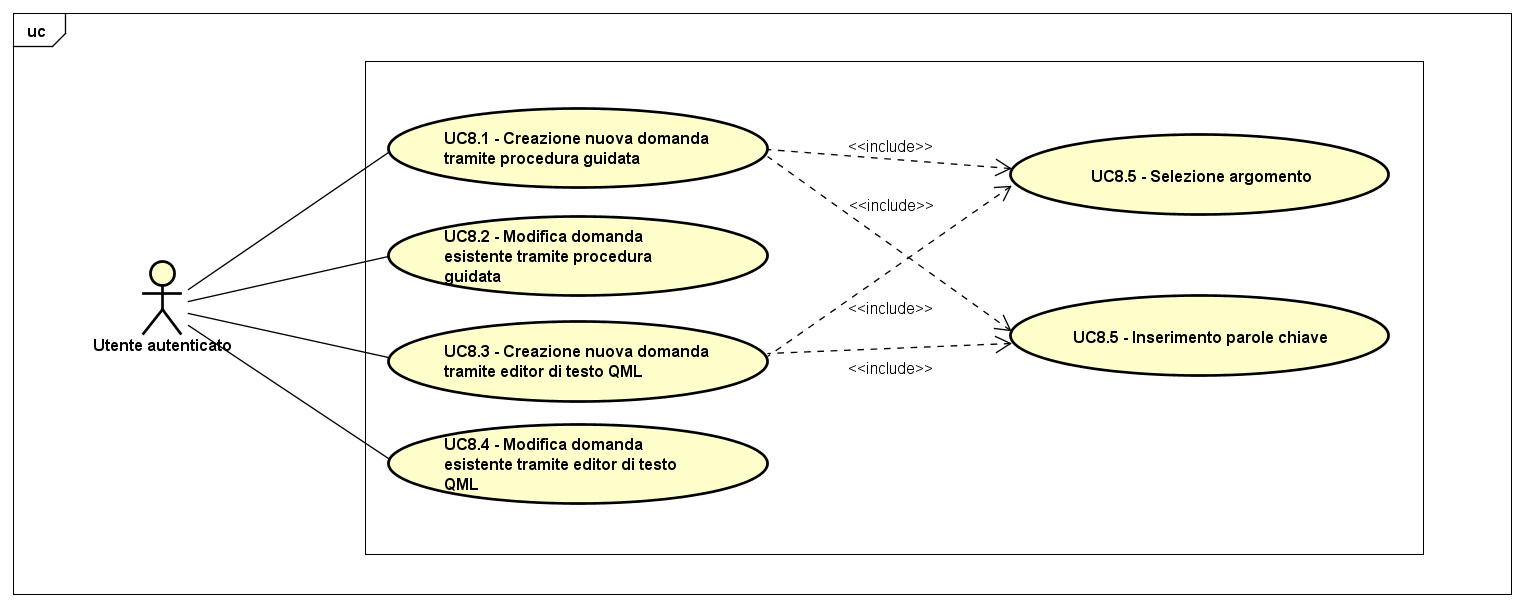
\includegraphics[scale=0.45,keepaspectratio]{UML/UC8.png}
		\caption{UC8: Gestione delle domande}
	\end{figure}
	\FloatBarrier
	\begin{itemize}
		\item
			\textbf{Attori}: utente autenticato, utente autenticato pro;
		\item		
			\textbf{Descrizione}: l'attore può creare e modificare domande;
		\item
			\textbf{Precondizione}: l'attore è autenticato presso il sistema; 
		\item
			\textbf{Postcondizione}: l'attore ha compiuto una delle operazioni appartenenti a questa funzionalità;
		\item
			\textbf{Scenario principale}:
	       		\begin{enumerate}
					\item
					L'attore crea una nuova domanda (UC8.1);
					\item
					L'attore modifica una domanda (UC8.2).
	 			\end{enumerate}
	\end{itemize}
\subsubsection{Caso d'uso UC8.1: Creazione nuova domanda}
	\label{UC8.1}
	\begin{figure}[h]
		\centering
			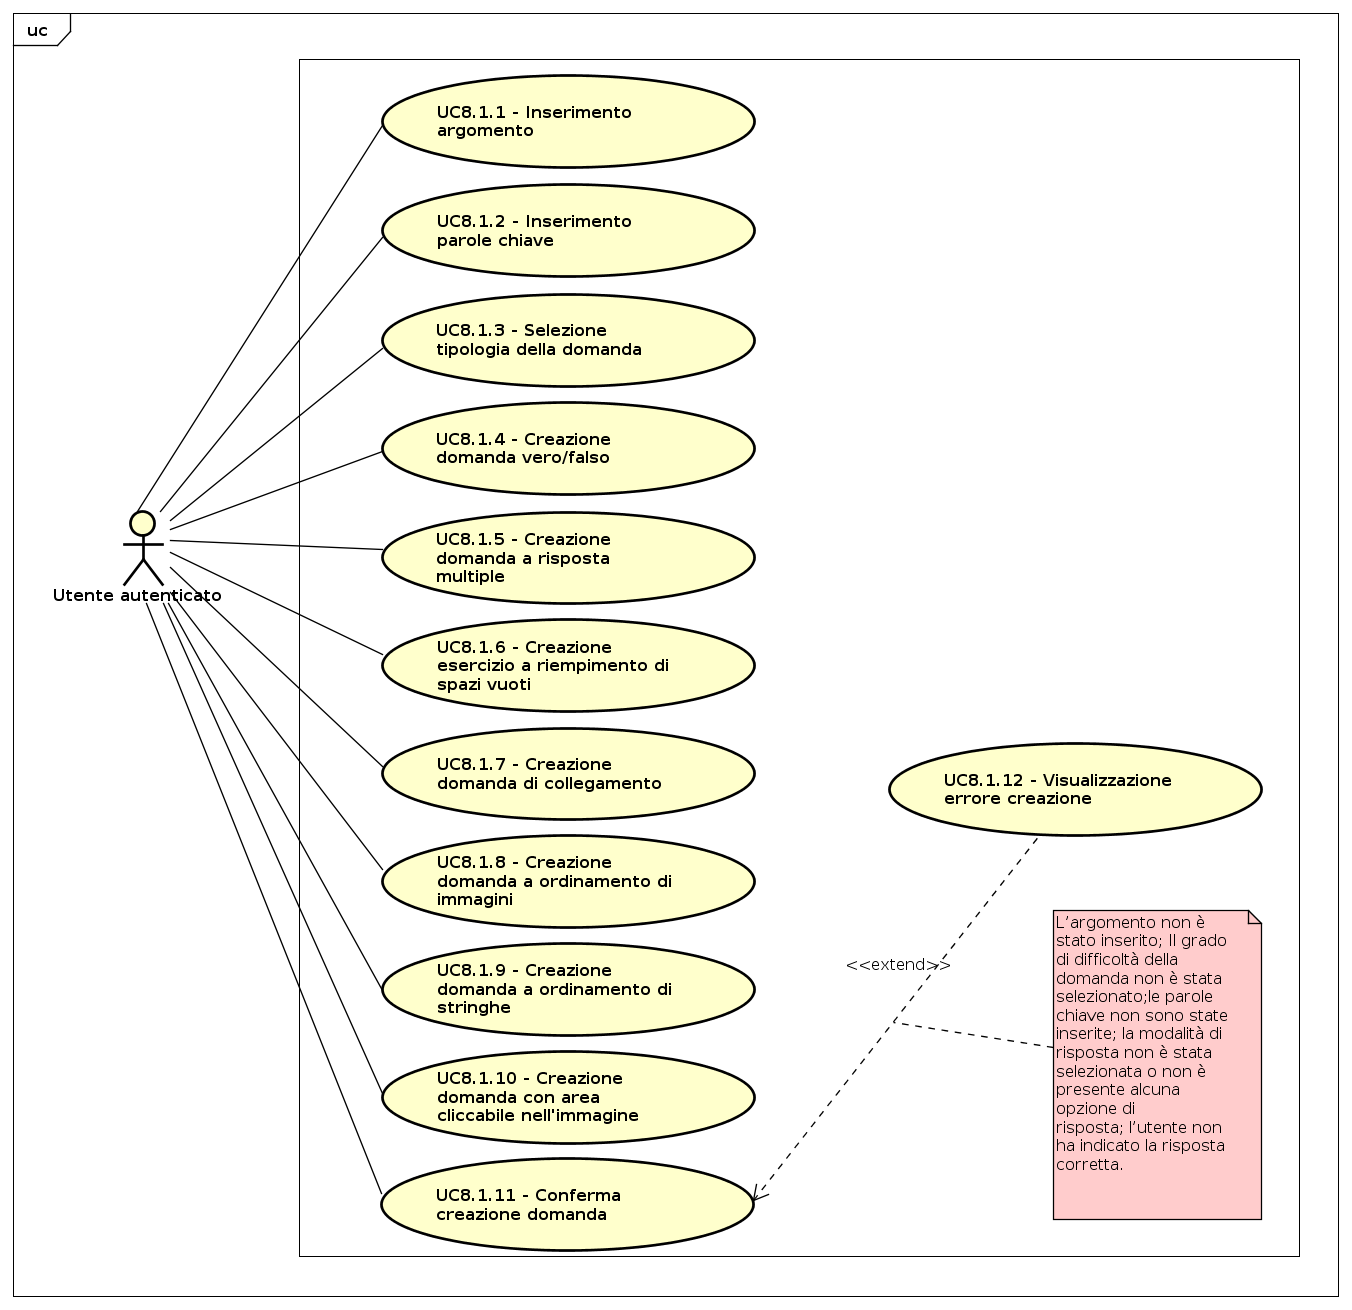
\includegraphics[scale=0.45,keepaspectratio]{UML/UC8_1.png}
		\caption{UC8.1: Creazione nuova domanda}
	\end{figure}
	\FloatBarrier
	\begin{itemize}
		\item
			\textbf{Attori}: utente autenticato, utente autenticato pro;
		\item		
			\textbf{Descrizione}: l'attore può creare una nuova domanda;
		\item
			\textbf{Precondizione}: l'attore ha selezionato la funzionalità di creazione domanda;
		\item
			\textbf{Postcondizione}: l'attore crea una domanda;		
		\item
			\textbf{Scenario principale}:
	       		\begin{enumerate}
					\item
					L'attore può inserire l'argomento relativo alla nuova domanda (UC8.1.1);
					\item
					L'attore può inserire le parole chiave relative alla nuova domanda (UC8.1.2);
					\item
					L'attore può selezionare la tipologia di domanda (UC8.1.3);
					\item
					L'attore può confermare la creazione della domanda (UC8.1.4).
	 			\end{enumerate}
	 	\item
			\textbf{Estensioni}: l'attore visualizza un messaggio d'errore relativo alla creazione della domanda (UC8.1.5);
	 	\item
	 		\textbf{Scenari alternativi}:
				\begin{itemize}
					\item 	
						L'argomento non è stato inserito;
					\item
						Le parole chiave non sono state inserite;
					\item
						La tipologia di domanda non è stata selezionata.	
				\end{itemize}
	\end{itemize}
	\subsubsection{Caso d'uso UC8.1.1: Selezione argomento}
	\begin{itemize}
		\item
			\textbf{Attori}: utente autenticato, utente autenticato pro;
		\item
			\textbf{Descrizione}: l'attore può indicare un argomento tra quelli presenti;
		\item		
			\textbf{Precondizione}: l'attore ha selezionato la funzionalità di creazione domanda;
		\item
			\textbf{Postcondizione}: l'attore ha selezionato un argomento;
		\item
			\textbf{Scenario principale}: l'attore seleziona l'argomento da assegnare alla nuova domanda.		
	\end{itemize}
		
	\subsubsection{Caso d'uso UC8.1.2: Inserimento parole chiave}
	\begin{itemize}
		\item
			\textbf{Attori}: utente autenticato, utente autenticato pro;
		\item
			\textbf{Descrizione}: l'attore può inserire le parole chiave relative alla nuova domanda per specificare più dettagliatamente l'argomento della domanda;
		\item		
			\textbf{Precondizione}: l'attore ha selezionato la funzionalità di creazione domanda;
		\item
			\textbf{Postcondizione}: l'attore ha selezionato delle parole chiave;
		\item
			\textbf{Scenario principale}: l'attore inserisce delle parole chiave relative alla nuova domanda.	
	\end{itemize}


	\subsubsection{Caso d'uso UC8.1.3: Selezione tipologia di domanda}
	\label{UC8.1.3}
	\begin{figure}[h]
		\centering
			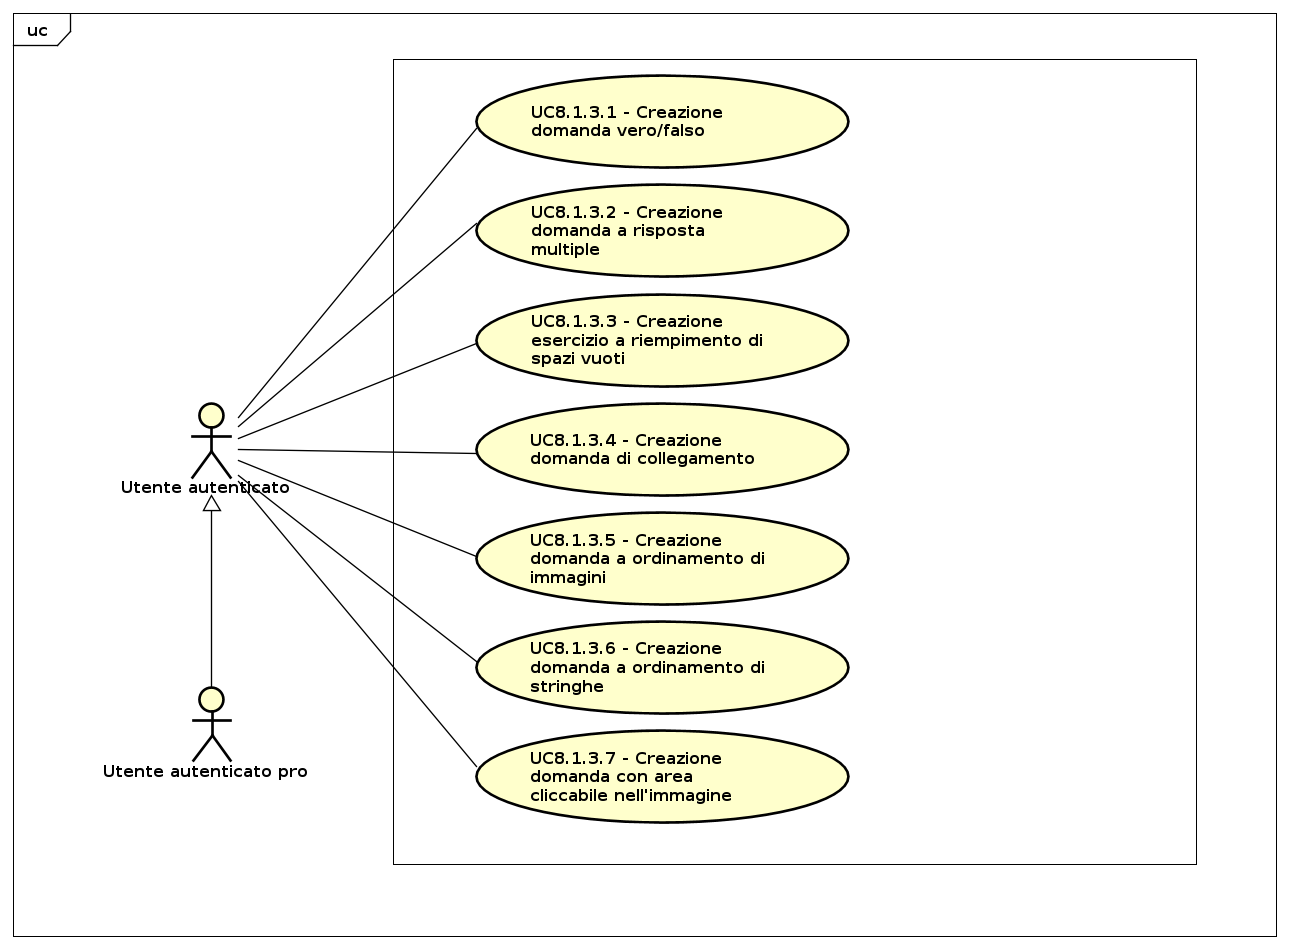
\includegraphics[scale=0.45,keepaspectratio]{UML/UC8_1_3.png}
		\caption{UC8.1.3: Selezione tipologia di domanda}
	\end{figure}
	\FloatBarrier
	\begin{itemize}
		\item
			\textbf{Attori}: utente autenticato, utente autenticato pro;
		\item
			\textbf{Descrizione}: l'attore può scegliere la tipologia di domanda che vuole inserire;
		\item		
			\textbf{Precondizione}: l'attore ha selezionato la funzionalità di creazione domanda;
		\item
			\textbf{Postcondizione}: l'utente ha selezionato la tipologia di domanda da inserire;
				\item \textbf{Scenario principale}: 
					\begin{enumerate}
					\item
					L'attore può richiamare il wizard per creare una domanda vero/falso (UC8.1.3.1);
					\item
					L'attore può richiamare il wizard per creare una domanda a risposta multipla (UC8.1.3.2);
					\item
					L'attore può richiamare il wizard per creare un esercizio a riempimento di spazi vuoti (UC8.1.3.3);
					\item
					L'attore può richiamare il wizard per creare una domanda di collegamento (UC8.1.3.4);
					\item
					L'attore può richiamare il wizard per creare una domanda a ordinamento di immagini (UC8.1.3.5);
					\item
					L'attore può richiamare il wizard per creare una domanda a ordinamento di stringhe (UC8.1.3.6);
					\item
					L'attore può richiamare il wizard per creare una domanda con area cliccabile nell'immagine (UC8.1.3.7).
	 			\end{enumerate}
	\end{itemize}

	%inclusione file latex wizard
\subsubsection{Caso d'uso UC8.1.3.1: Creazione domanda vero/falso}
	\begin{itemize}
		\item
			\textbf{Attori}: utente autenticato, utente autenticato pro;
		\item		
			\textbf{Descrizione}: lo scopo di questa funzionalità è offrire agli attori la possibilità di creare domande vero/falso;
		\item
			\textbf{Precondizione}: gli attori hanno selezionato la seguente funzionalità; 
		\item
			\textbf{Postcondizione}: gli attori hanno creato una domanda vero/falso;
		\item
			\textbf{Scenario principale}:
	       		\begin{enumerate}
	       			\item
	       			Gli attori devono compilare il campo dati destinato alla scrittura del testo della domanda (UC8.1.3.1.1)
	       			\item
	       			Gli attori possono inserire una immagine relativa al testo della domanda (UC8.1.3.1.2)
					\item
					Gli attori devono indicare la risposta corretta tramite uno strumento di selezione |(UC8.1.3.1.3).
	 			\end{enumerate}
	\end{itemize}

\subsubsection{Caso d'uso UC8.1.3.1.1: Inserimento testo della domanda}
	\begin{itemize}
		\item
			\textbf{Attori}: utente autenticato, utente autenticato pro;
		\item		
			\textbf{Descrizione}: lo scopo di questa funzionalità è offrire agli attori la possibilità di inserire il testo della domanda;
		\item
			\textbf{Precondizione}: gli attori hanno selezionato la modalità di creazione di una domanda vero/falso; 
		\item
			\textbf{Postcondizione}: gli attori hanno inserito il testo della domanda;
		\item
			\textbf{Scenario principale}: gli attori inseriscono il testo della domanda. 
	 			
	\end{itemize}
	
\subsubsection{Caso d'uso UC8.1.3.1.2: Inserimento immagine}
	\begin{itemize}
		\item
			\textbf{Attori}: utente autenticato, utente autenticato pro;
		\item		
			\textbf{Descrizione}: lo scopo di questa funzionalità è offrire agli attori la possibilità di inserire un'immagine relativa al testo della domanda;
		\item
			\textbf{Precondizione}: gli attori hanno selezionato la modalità di creazione di una domanda vero/falso; 
		\item
			\textbf{Postcondizione}: gli attori hanno inserito l'immagine;
		\item
			\textbf{Scenario principale}: gli attori inseriscono l'immagine. 	
	\end{itemize}
	

\subsubsection{Caso d'uso UC8.1.3.1.3: Selezione risposta corretta}
	\begin{itemize}
		\item
			\textbf{Attori}: utente autenticato, utente autenticato pro;
		\item		
			\textbf{Descrizione}: lo scopo di questa funzionalità è offrire agli attori la possibilità, tramite uno strumento di selezione, di indicare la risposta corretta;
		\item
			\textbf{Precondizione}: gli attori hanno selezionato la modalità di creazione di una domanda vero/falso; 
		\item
			\textbf{Postcondizione}: gli attori hanno selezionato la risposta corretta;
		\item
			\textbf{Scenario principale}: gli attori indicano la risposta corretta tramite uno strumento di selezione. 
	 			
	\end{itemize}
	

	

\subsubsection{Caso d'uso UC8.1.3.2: Creazione domanda a risposta multipla}
	\label{UC8.1.3.2}
	\begin{figure}[h]
		\centering
			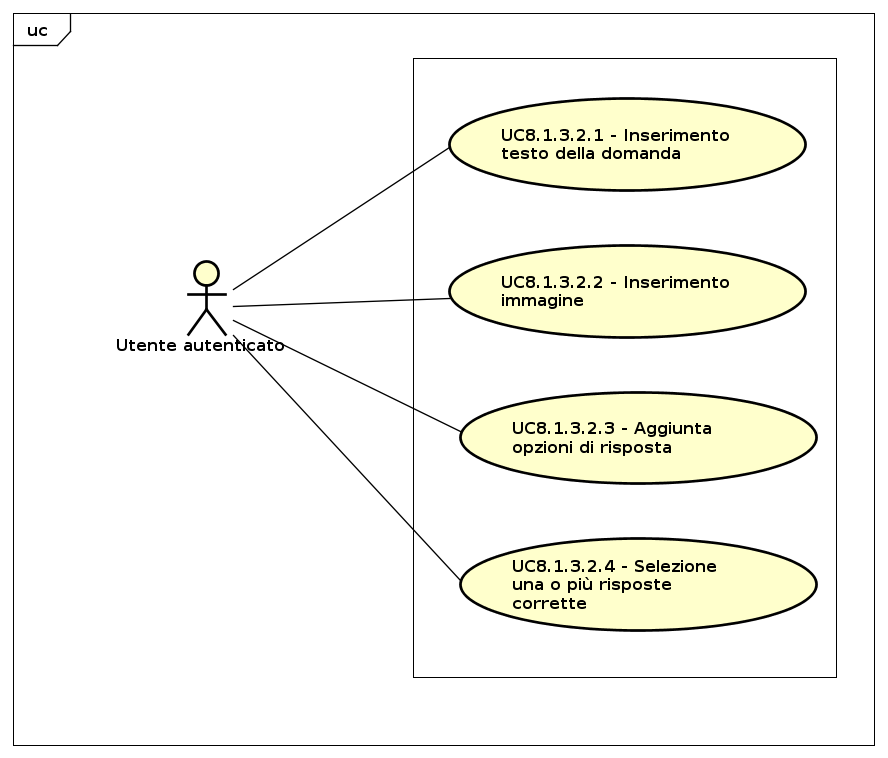
\includegraphics[scale=0.45,keepaspectratio]{UML/UC8_1_3_2.png}
		\caption{UC8.1.3.2: Creazione domanda a risposta multipla}
	\end{figure}
	\FloatBarrier
	\begin{itemize}
		\item
			\textbf{Attori}: utente autenticato, utente autenticato pro;
		\item		
			\textbf{Descrizione}: l'attore può utilizzare la procedura guidata per la creazione di una domanda a risposta multipla;
		\item
			\textbf{Precondizione}: l'attore ha selezionato la funzionalità di creazione di una domanda a risposta multipla;
		\item
			\textbf{Postcondizione}: l'attore ha creato una domanda a risposta multipla;
		\item
			\textbf{Scenario principale}:
	       		\begin{enumerate}
	       			\item
	       			L'attore può inserire il testo della domanda (UC8.1.3.2.1);
	       			\item
	       			L'attore può inserire un'immagine relativa al testo della domanda (UC8.1.3.2.2);
	       			\item
	       			L'attore può aggiungere almeno due opzioni di risposta (UC8.1.3.2.3);
					\item
					L'attore può indicare una o più risposte corrette (UC8.1.3.2.4).
	 			\end{enumerate}
	\end{itemize}

\subsubsection{Caso d'uso UC8.1.3.2.1: Inserimento testo della domanda}
	\begin{itemize}
		\item
			\textbf{Attori}: utente autenticato, utente autenticato pro;
		\item		
			\textbf{Descrizione}: l'attore può inserire il testo della domanda;
		\item
			\textbf{Precondizione}: l'attore ha selezionato la funzionalità di creazione di una domanda a risposta multipla; 
		\item
			\textbf{Postcondizione}: l'attore ha inserito il testo della domanda;
		\item
			\textbf{Scenario principale}: l'attore inserisce il testo della domanda. 
	 			
	\end{itemize}
	
\subsubsection{Caso d'uso UC8.1.3.2.2: Inserimento immagine}
	\begin{itemize}
		\item
			\textbf{Attori}: utente autenticato, utente autenticato pro;
		\item		
			\textbf{Descrizione}: l'attore può inserire un'immagine relativa al testo della domanda;
		\item
			\textbf{Precondizione}: l'attore ha selezionato la funzionalità di creazione di una domanda a risposta multipla; 
		\item
			\textbf{Postcondizione}: l'attore ha inserito un'immagine relativa al testo della domanda;
		\item
			\textbf{Scenario principale}: l'attore inserisce l'immagine.						
	\end{itemize}


	
\subsubsection{Caso d'uso UC8.1.3.2.3: Aggiunta opzioni di risposta}
	\label{UC8.1.3.2.3}
	\begin{figure}[h]
		\centering
			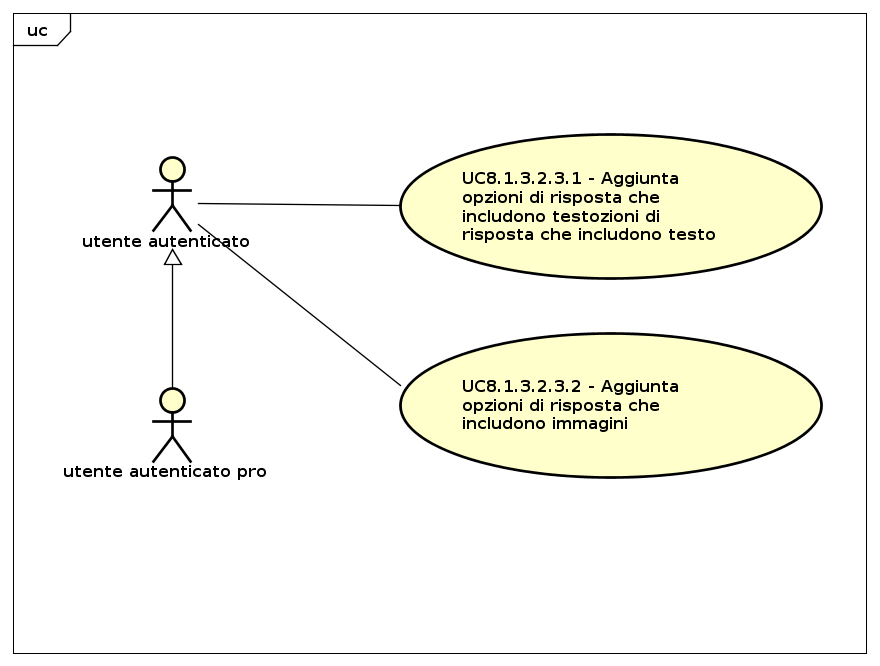
\includegraphics[scale=0.45,keepaspectratio]{UML/UC8_1_3_2_3.png}
		\caption{UC8.1.3.2.3: Aggiunta opzioni di risposta}
	\end{figure}
	\FloatBarrier
	\begin{itemize}
		\item
			\textbf{Attori}: utente autenticato, utente autenticato pro;
		\item		
			\textbf{Descrizione}: l'attore può aggiungere almeno due opzioni di risposta;
		\item
			\textbf{Precondizione}: l'attore ha selezionato la funzionalità di creazione di una domanda a risposta multipla;
		\item
			\textbf{Postcondizione}: l'attore ha aggiunto due o più opzioni di risposta;
		\item
			\textbf{Scenario principale}:
	       		\begin{enumerate}
	       			\item
	       			L'attore può aggiungere opzioni di risposta che includono testo (UC8.1.3.2.3.1);
					\item
					L'attore può aggiungere opzioni di risposta che includono immagini (UC8.1.3.2.3.2).
	 			\end{enumerate}
	\end{itemize}	

\subsubsection{Caso d'uso UC8.1.3.2.3.1: Aggiunta opzioni di risposta che includono testo}
	\begin{itemize}
		\item
			\textbf{Attori}: utente autenticato, utente autenticato pro;
		\item		
			\textbf{Descrizione}: l'attore può aggiungere almeno due opzioni di risposta che includono testo;
		\item
			\textbf{Precondizione}: l'attore ha selezionato la funzionalità di creazione di una domanda a risposta multipla;
		\item
			\textbf{Postcondizione}: l'attore ha aggiunto due o più opzioni di risposta che includono testo;
		\item
			\textbf{Scenario principale}: l'attore aggiunge due o più opzioni che includono testo.				
	\end{itemize}	

\subsubsection{Caso d'uso UC8.1.3.2.3.2: Aggiunta opzioni di risposta che includono immagini}
	\begin{itemize}
		\item
			\textbf{Attori}: utente autenticato, utente autenticato pro;
		\item		
			\textbf{Descrizione}: l'attore può aggiungere almeno due opzioni di risposta che includono immagini;
		\item
			\textbf{Precondizione}: l'attore ha selezionato la funzionalità di creazione di una domanda a risposta multipla;
		\item
			\textbf{Postcondizione}: l'attore ha aggiunto due o più opzioni di risposta che includono immagini;
		\item
			\textbf{Scenario principale}: l'attore aggiunge due o più opzioni che includono immagini. 				
	\end{itemize}	
		
\subsubsection{Caso d'uso UC8.1.3.2.4: Selezione una o più risposte corrette}
	\begin{itemize}
		\item
			\textbf{Attori}: utente autenticato, utente autenticato pro;
		\item		
			\textbf{Descrizione}: l'attore può indicare una o più risposte corrette;
		\item
			\textbf{Precondizione}: l'attore ha selezionato la funzionalità di creazione di una domanda a risposta multipla;
		\item
			\textbf{Postcondizione}: l'attore ha selezionato una o più risposte corrette;
		\item
			\textbf{Scenario principale}: l'attore indica una o più risposte corrette. 			
	\end{itemize}
\subsubsection{Caso d'uso UC8.1.3.3: Creazione esercizi di riempimento degli spazi vuoti}
	\label{UC8.1.3.3}
	\begin{figure}[h]
		\centering
			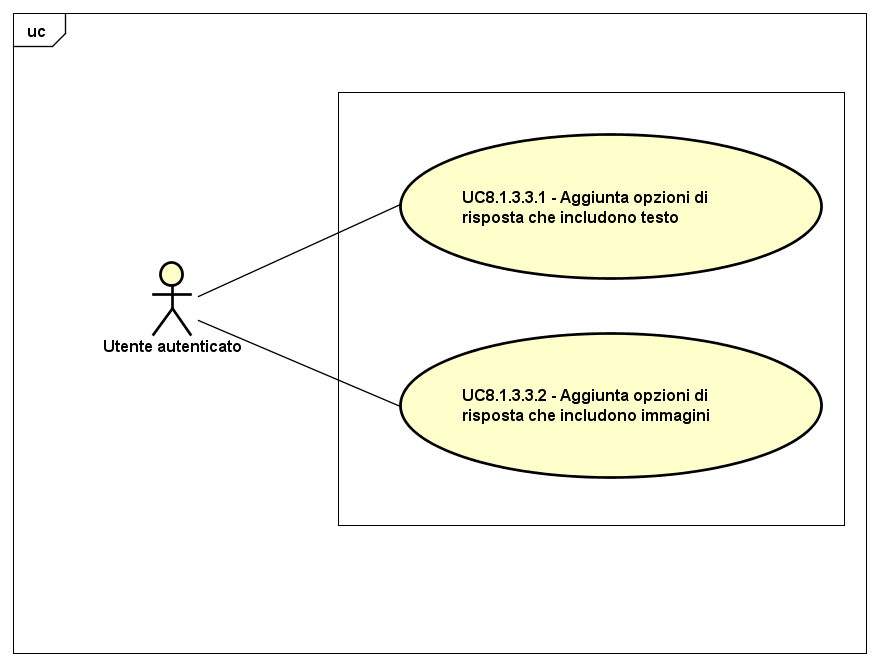
\includegraphics[scale=0.45,keepaspectratio]{UML/UC8_1_3_3.png}
		\caption{UC8.1.3.3: Creazione esercizi di riempimento degli spazi vuoti}
	\end{figure}
	\FloatBarrier
	\begin{itemize}
		\item
			\textbf{Attori}: utente autenticato, utente autenticato pro;
		\item		
			\textbf{Descrizione}: l'attore può creare esercizi di riempimento degli spazi vuoti;
		\item
			\textbf{Precondizione}: l'attore ha selezionato la seguente funzionalità; 
		\item
			\textbf{Postcondizione}: l'attore ha creato un esercizio di riempimento degli spazi vuoti;
		\item
			\textbf{Scenario principale}:
	       		\begin{enumerate}
	       			\item
	       			L'attore può compilare il campo dati destinato alla scrittura del testo dell'esercizio (UC8.1.3.3.1);
	       			\item
	       			L'attore può indicare le parole che saranno sostituite con degli spazi vuoti dal sistema (UC8.1.3.3.2).
	 			\end{enumerate}
	\end{itemize}
	
\subsubsection{Caso d'uso UC8.1.3.3.1: Scrittura testo dell'esercizio}
	\begin{itemize}
		\item
			\textbf{Attori}: utente autenticato, utente autenticato pro;
		\item		
			\textbf{Descrizione}: l'attore può inserire il testo dell'esercizio di riempimento;
		\item
			\textbf{Precondizione}: l'attore può creare un esercizio di riempimento degli spazi vuoti; 
		\item
			\textbf{Postcondizione}: l'attore ha compilato il campo dati dedicato alla scrittura del testo dell'esercizio di riempimento;
		\item
			\textbf{Scenario principale}: l'attore compila il campo dati dedicato alla scrittura del testo dell'esercizio di riempimento.
	\end{itemize}


\subsubsection{Caso d'uso UC8.1.3.3.2: Indicazione parole da oscurare}
	\begin{itemize}
		\item
			\textbf{Attori}: utente autenticato, utente autenticato pro;
		\item		
			\textbf{Descrizione}: l'attore può indicare le parole che saranno sostituite con degli spazi vuoti;
		\item
			\textbf{Precondizione}: l'attore ha inserito il testo dell'esercizio; 
		\item
			\textbf{Postcondizione}: l'attore ha indicato le parole che saranno sostituite con degli spazi vuoti;
		\item
			\textbf{Scenario principale}: l'attore indica le parole che verranno oscurate dal sistema.
	\end{itemize}
\subsubsection{Caso d'uso UC8.1.3.4: Creazione domanda di collegamento}
\label{UC8.1.3.4}
\begin{figure}[h]
	\centering
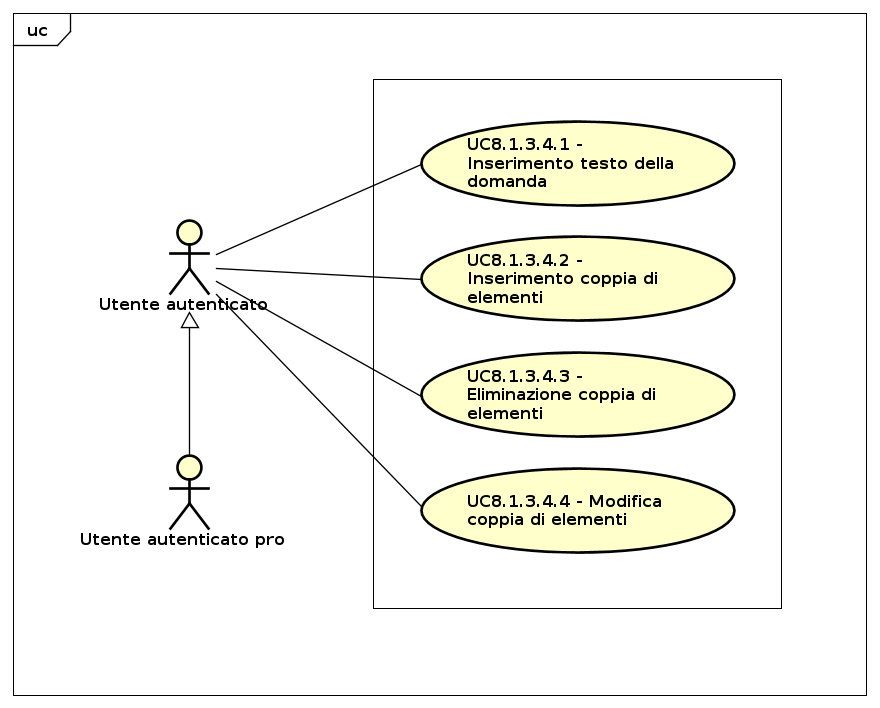
\includegraphics[scale=0.5,keepaspectratio]{UML/UC8_1_3_4.png}
	\caption{Caso d'uso UC8.1.3.4: Creazione domanda di collegamento}
\end{figure}
\FloatBarrier
\begin{itemize}
	\item \textbf{Attori}: \uau, \uaupro;
	\item \textbf{Descrizione}: l'attore utilizza la procedura guidata per la creazione di una domanda di tipo collegamento. 
	\item \textbf{Precondizione}: l'attore ha scelto l'opzione "Creazione domanda di collegamento" nelle scelte possibili nel caso d'uso UC8.1.3;
	\item \textbf{Postcondizione}: l'attore ha completato tutti i campi necessari per la creazione di una domanda di tipo collegamento. L'attore deve inserire almeno due coppie per rispettare la postcondizione;
	\item \textbf{Scenario principale}: 
		\begin{enumerate}
			\item L'attore inserisce una coppia di elementi (UC8.1.3.4.1);
			\item L'attore può eliminare una coppia di elementi appena inserita (UC8.1.3.4.2);
			\item L'attore può modificare una coppia di elementi (UC8.1.3.4.3).
		\end{enumerate}
	\item \textbf{Scenari alternativi}: se non ci sono almeno due coppie presenti nella lista delle coppie l'utente deve inserire una nuova coppia di elementi.
\end{itemize}

	\subsubsection{Caso d'uso UC8.1.3.4.1: Inserimento coppia di elementi}
	\label{UC8.1.3.4.1}
	\begin{figure}[h]
		\centering
		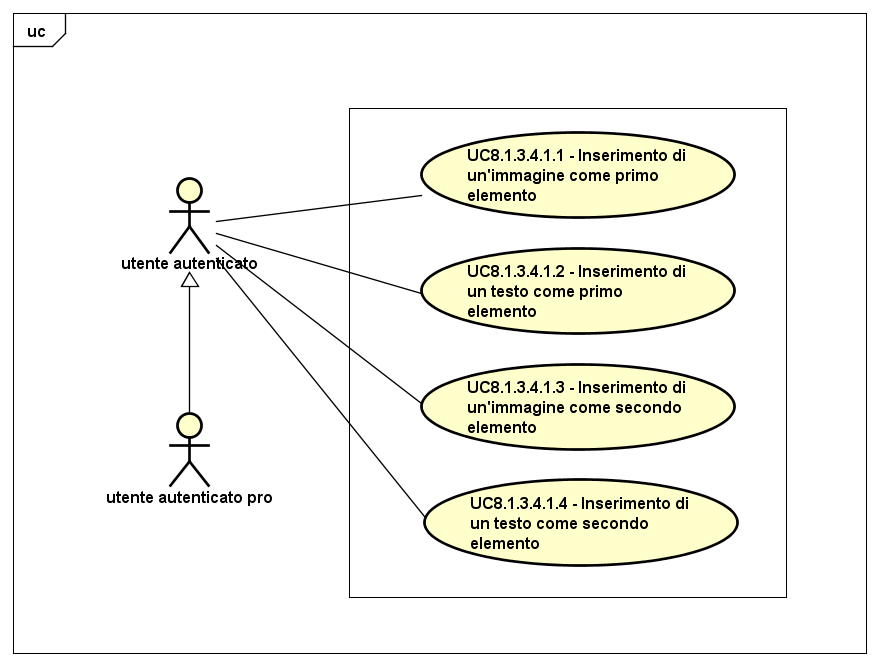
\includegraphics[scale=0.5,keepaspectratio]{UML/UC8_1_3_4_1.png}
		\caption{Caso d'uso UC8.1.3.4.1: Inserimento coppia di elementi}
	\end{figure}
	\FloatBarrier
	\begin{itemize}
		\item \textbf{Attori}: \uau, \uaupro;
		\item \textbf{Descrizione}: l'attore inserisce una coppia di elementi e questi possono essere sia immagini che testo o combinazioni di questi. Un coppia una volta creata sarà già soluzione di essa stessa: il primo elemento dovrà essere collegato con il secondo o viceversa. 
		\item \textbf{Precondizione}: l'attore ha scelto l'opzione "Inserimento coppia di elementi" nelle scelte possibili nel caso d'uso UC8.1.3.4;
		\item \textbf{Postcondizione}: l'attore ha inserito una coppia di elementi nella lista di coppie di elementi; 
		\item \textbf{Scenario principale}: 
		\begin{enumerate}
			\item L'attore inserisce come primo elemento un'immagine (UC8.1.3.4.1.1);
			\item L'attore inserisce come primo elemento un testo (UC8.1.3.4.1.2);
			\item L'attore inserisce come secondo elemento un'immagine (UC8.1.3.4.1.3);
			\item L'attore inserisce come secondo elemento un testo (UC8.1.3.4.1.4).	
		\end{enumerate}
	\end{itemize}
	
		\subsubsection{Caso d'uso UC8.1.3.4.1.1: Inserimento di un'immagine come primo elemento}
		\label{UC8.1.3.4.1.1}
		\begin{itemize}
			\item \textbf{Attori}: \uau, \uaupro;
			\item \textbf{Descrizione}: l'attore decide di inserire come primo elemento della coppia un'immagine;
			\item \textbf{Precondizione}: l'attore ha scelto l'opzione "Inserimento di un'immagine come primo elemento" nelle scelte possibili nel caso d'uso UC8.1.3.4.1 e non ha già scelto l'opzione presentata dall'use case UC8.1.3.4.1.2;
			\item \textbf{Postcondizione}: l'utente ha inserito come primo elemento un'immagine;
			\item \textbf{Scenario principale}: l'attore carica un'immagine come primo elemento della coppia;  
			\item \textbf{Scenari alternativi}: l'attore non può selezionare il seguente campo se è già stata utilizzata l'opzione proposta dall'use case UC8.1.3.4.1.2. Viene così rimandato all'use case UC8.1.3.4.1;
		\end{itemize}
		
		\subsubsection{Caso d'uso UC8.1.3.4.1.2: Inserimento di un testo come primo elemento}
		\label{UC8.1.3.4.1.2}
		\begin{itemize}
			\item \textbf{Attori}: \uau, \uaupro;
			\item \textbf{Descrizione}: l'attore decide di inserire come primo elemento della coppia un testo;
			\item \textbf{Precondizione}: l'attore ha scelto l'opzione "Inserimento di un testo come primo elemento" nelle scelte possibili nel caso d'uso UC8.1.3.4.1 e non ha già scelto l'opzione presentata dall'use case UC8.1.3.4.1.1;
			\item \textbf{Postcondizione}: l'utente ha inserito come primo elemento un testo;
			\item \textbf{Scenario principale}: l'attore inserisce del testo come primo elemento della coppia ;  
			\item \textbf{Scenari alternativi}: l'attore non può selezionare il seguente campo se è già stata utilizzata l'opzione proposta dall'use case UC8.1.3.4.1.1. Viene così rimandato all'use case UC8.1.3.4.1;
		\end{itemize}
		
			\subsubsection{Caso d'uso UC8.1.3.4.1.3: Inserimento di un'immagine come secondo elemento}
		\label{UC8.1.3.4.1.3}
		\begin{itemize}
			\item \textbf{Attori}: \uau, \uaupro;
			\item \textbf{Descrizione}: l'attore decide di inserire come secondo elemento della coppia un'immagine;
			\item \textbf{Precondizione}: l'attore ha scelto l'opzione "Inserimento di un'immagine come secondo elemento" nelle scelte possibili nel caso d'uso UC8.1.3.4.1 e non ha già scelto l'opzione presentata dall'use case UC8.1.3.4.1.4;
			\item \textbf{Postcondizione}: l'utente ha inserito come secondo elemento un'immagine;
			\item \textbf{Scenario principale}: l'attore carica un'immagine come secondo elemento della coppia;  
			\item \textbf{Scenari alternativi}: l'attore non può selezionare il seguente campo se è già stata utilizzata l'opzione proposta dall'use case UC8.1.3.4.1.4. Viene così rimandato all'use case UC8.1.3.4.1;
		\end{itemize}
		
		\subsubsection{Caso d'uso UC8.1.3.4.1.4: Inserimento di un testo come secondo elemento}
		\label{UC8.1.3.4.1.4}
		\begin{itemize}
			\item \textbf{Attori}: \uau, \uaupro;
			\item \textbf{Descrizione}: l'attore decide di inserire come secondo elemento della coppia un testo;
			\item \textbf{Precondizione}: l'attore ha scelto l'opzione "Inserimento di un testo come secondo elemento" nelle scelte possibili nel caso d'uso UC8.1.3.4.1 e non ha già scelto l'opzione presentata dall'use case UC8.1.3.4.1.3;
			\item \textbf{Postcondizione}: l'utente ha inserito come secondo elemento un'immagine;
			\item \textbf{Scenario principale}: l'attore inserisce del testo come secondo elemento della coppia;  
			\item \textbf{Scenari alternativi}: l'attore non può selezionare il seguente campo se è già stata utilizzata l'opzione proposta dall'use case UC8.1.3.4.1.3. Viene così rimandato all'use case UC8.1.3.4.1;
		\end{itemize}
	
	\subsubsection{Caso d'uso UC8.1.3.4.2: Eliminazione coppia di elementi}
	\label{UC8.1.3.4.2}
	\begin{figure}[h]
		\centering
		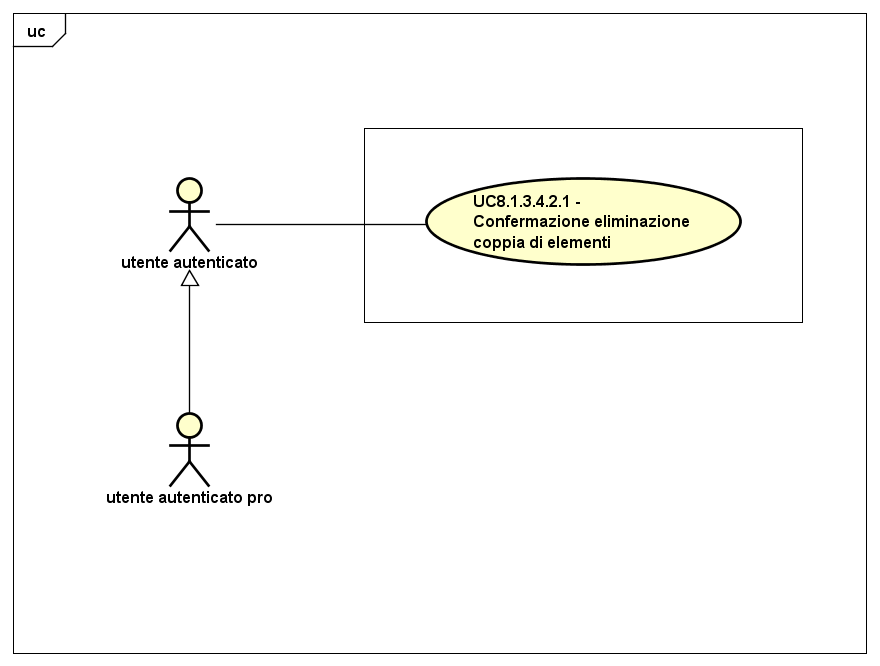
\includegraphics[scale=0.5,keepaspectratio]{UML/UC8_1_3_4_2.png}
		\caption{Caso d'uso UC8.1.3.4.2: Eliminazione coppia di elementi}
	\end{figure}
	\FloatBarrier
	\begin{itemize}
		\item \textbf{Attori}: \uau, \uaupro;
		\item \textbf{Descrizione}: l'utente decide di eliminare una coppia di elementi dalla lista di coppie di elementi;
		\item \textbf{Precondizione}: l'attore ha scelto l'opzione "Eliminazione coppia di elementi" nelle scelte possibili nel caso d'uso UC8.1.3.4;
		\item \textbf{Postcondizione}: l'attore ha eliminato, dalla lista delle coppie di elementi, una coppia;
		\item \textbf{Scenario principale}: l'attore deve confermare di voler eliminare una coppia di elementi (UC8.1.3.4.2.1); 
	\end{itemize}

		\subsubsection{Caso d'uso UC8.1.3.4.2.1: Confermazione eliminazione coppia di elementi}
		\label{UC8.1.3.4.2.1}
		\begin{itemize}
			\item \textbf{Attori}: \uau, \uaupro;
			\item \textbf{Descrizione}: l'attore deve confermare di voler eliminare la coppia di elementi;
			\item \textbf{Precondizione}: l'attore ha scelto l'opzione "Confermazione eliminazione coppia di elementi" nelle scelte possibili nel caso d'uso UC8.1.3.4.2;
			\item \textbf{Postcondizione}: l'attore ha confermato di voler eliminare la coppia di elementi;
			\item \textbf{Scenario principale}: l'attore conferma di voler eliminare la coppia di elementi;
			\item \textbf{Scenari alternativi}: l'attore non conferma di voler eliminare la coppia di elementi; 
		\end{itemize}

	\subsubsection{Caso d'uso UC8.1.3.4.3: Modifica coppia di elementi}
	\label{UC8.1.3.4.3}
	\begin{figure}[h]
		\centering
		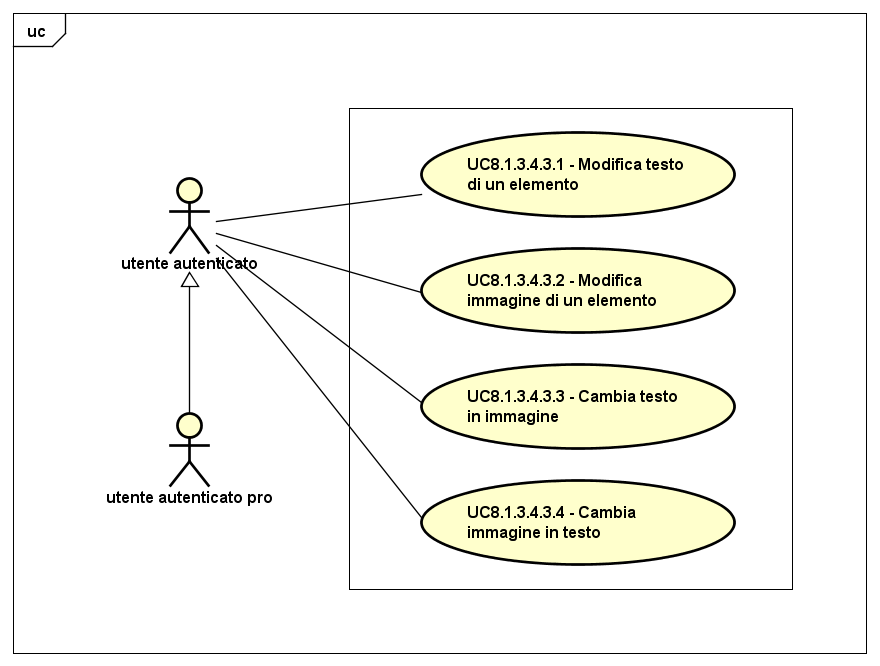
\includegraphics[scale=0.5,keepaspectratio]{UML/UC8_1_3_4_3.png}
		\caption{Caso d'uso UC8.1.3.4.3: Modifica coppia di elementi}
	\end{figure}
	\FloatBarrier
	\begin{itemize}
		\item \textbf{Attori}: \uau, \uaupro;
		\item \textbf{Descrizione}: l'attore modifica una coppia di elementi;
		\item \textbf{Precondizione}: l'attore ha scelto l'opzione "Modifica coppia di elementi" nelle scelte possibili nel caso d'uso UC8.1.3.4;
		\item \textbf{Postcondizione}: l'attore ha modificato una coppia di elementi nella lista di coppie di elementi; 
		\item \textbf{Scenario principale}: 
		\begin{enumerate}
			\item L'attore modifica un elemento cambiandone il testo (UC8.1.3.4.1.1);
			\item L'attore modifica un elemento cambiandone l'immagine (UC8.1.3.4.1.2);
			\item L'attore modifica un elemento facendolo passare da testo ad immagine (UC8.1.3.4.1.3);
			\item L'attore modifica un elemento facendolo passare da immagine a testo (UC8.1.3.4.1.4).	
		\end{enumerate}
	\end{itemize}
	
		\subsubsection{Caso d'uso UC8.1.3.4.3.1: Modifica testo di un elemento}
		\label{UC8.1.3.4.3.1}
		\begin{itemize}
			\item \textbf{Attori}: \uau, \uaupro;
			\item \textbf{Descrizione}: l'attore decide di modificare il testo di un elemento;
			\item \textbf{Precondizione}: l'attore ha scelto l'opzione "Modifica testo di un elemento" nelle scelte possibili nel caso d'uso UC8.1.3.4.3;
			\item \textbf{Postcondizione}: l'utente ha modificato il testo di un elemento;
			\item \textbf{Scenario principale}: l'attore modifica il testo di un elemento;  
		\end{itemize}
		
		\subsubsection{Caso d'uso UC8.1.3.4.3.2: Modifica immagine di un elemento}
		\label{UC8.1.3.4.3.2}
		\begin{itemize}
			\item \textbf{Attori}: \uau, \uaupro;
			\item \textbf{Descrizione}: l'attore decide di caricare un'altra immagine per un elemento;
			\item \textbf{Precondizione}: l'attore ha scelto l'opzione "Modifica immagine di un elemento" nelle scelte possibili nel caso d'uso UC8.1.3.4.3;
			\item \textbf{Postcondizione}: l'utente ha caricato un'altra immagine per un elemento;
			\item \textbf{Scenario principale}: l'attore carica un'altra immagine per un elemento;
		\end{itemize}
		
		\subsubsection{Caso d'uso UC8.1.3.4.3.3: Cambia testo in immagine}
		\label{UC8.1.3.4.3.3}
		\begin{itemize}
			\item \textbf{Attori}: \uau, \uaupro;
			\item \textbf{Descrizione}: l'attore decide di modificare un elemento facendolo diventare un'immagine al posto di un testo;
			\item \textbf{Precondizione}: l'attore ha scelto l'opzione "Cambia testo in immagine" nelle scelte possibili nel caso d'uso UC8.1.3.4.3;
			\item \textbf{Postcondizione}: l'utente ha fatto diventare un'immagine un elemento che prima era un testo;
			\item \textbf{Scenario principale}: l'attore inserisce un'immagine come modifica dell'elemento;  
		\end{itemize}
		
		\subsubsection{Caso d'uso UC8.1.3.4.3.4: Cambia immagine in testo}
		\label{UC8.1.3.4.3.4}
		\begin{itemize}
			\item \textbf{Attori}: \uau, \uaupro;
			\item \textbf{Descrizione}: l'attore decide di modificare un elemento facendolo diventare un testo al posto di un'immagine;
			\item \textbf{Precondizione}: l'attore ha scelto l'opzione "Cambia immagine in testo" nelle scelte possibili nel caso d'uso UC8.1.3.4.3;
			\item \textbf{Postcondizione}: l'utente ha fatto diventare un testo un elemento che prima era un'immagine;
			\item \textbf{Scenario principale}: l'attore inserisce del testo come modifica dell'elemento;  
		\end{itemize}

\subsubsection{Caso d'uso UC8.1.3.5: Creazione domanda a ordinamento di immagini}
\label{UC8.1.3.5}
	\begin{figure}[h]
		\centering
			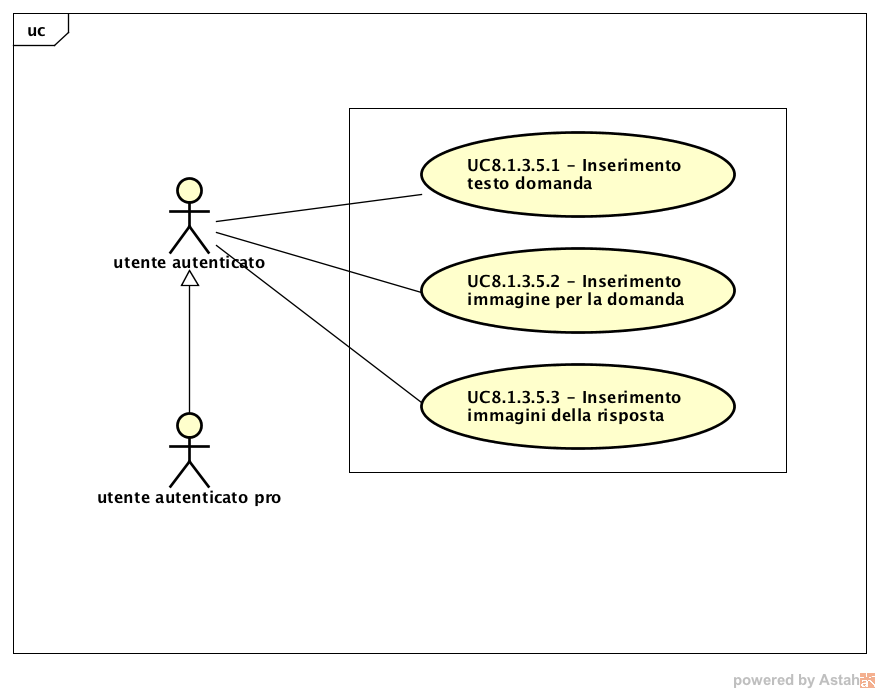
\includegraphics[scale=0.45,keepaspectratio]{UML/UC8_1_3_5.png}
		\caption{UC8.1.3.5: Creazione domanda a ordinamento di immagini}
	\end{figure}
	\FloatBarrier
\begin{itemize}
	\item\textbf{Attori}: utente autenticato, utente autenticato pro;
	\item\textbf{Descrizione}: l'attore può utilizzare la procedura guidata per la creazione di una domanda a ordinamento di immagini;
	\item\textbf{Precondizione}: l'attore ha selezionato la funzionalità di creazione di una domanda a ordinamento di immagini; 
	\item \textbf{Postcondizione}: l'attore ha creato una domanda a ordinamento di immagini;
	\item\textbf{Scenario principale}:
	\begin{itemize}
		\item L'attore può inserire il testo della domanda (UC8.1.3.5.1);
		\item L'attore può inserire un'immagine relativa al testo della domanda (UC8.1.3.5.2);
		\item L'attore può inserire le immagini della sequenza che costituirà la risposta (UC8.1.3.5.3).
	\end{itemize}
\end{itemize}

\subsubsection{Caso d'uso UC8.1.3.5.1: Inserimento testo domanda}
\begin{itemize}
	\item\textbf{Attori}: utente autenticato, utente autenticato pro;
	\item\textbf{Descrizione}: l'attore può inserire il testo della domanda;
	\item\textbf{Precondizione}: l'attore ha selezionato la funzionalità di creazione della domanda a ordinamento di immagini; 
	\item \textbf{Postcondizione}: l'attore ha inserito il testo della domanda;
	\item\textbf{Scenario principale}: l'attore inserisce il testo della domanda. 
\end{itemize}

\subsubsection{Caso d'uso UC8.1.3.5.2: Inserimento immagine per testo domanda}
\label{UC8.1.3.5.2}
\begin{figure}[h]
	\centering
	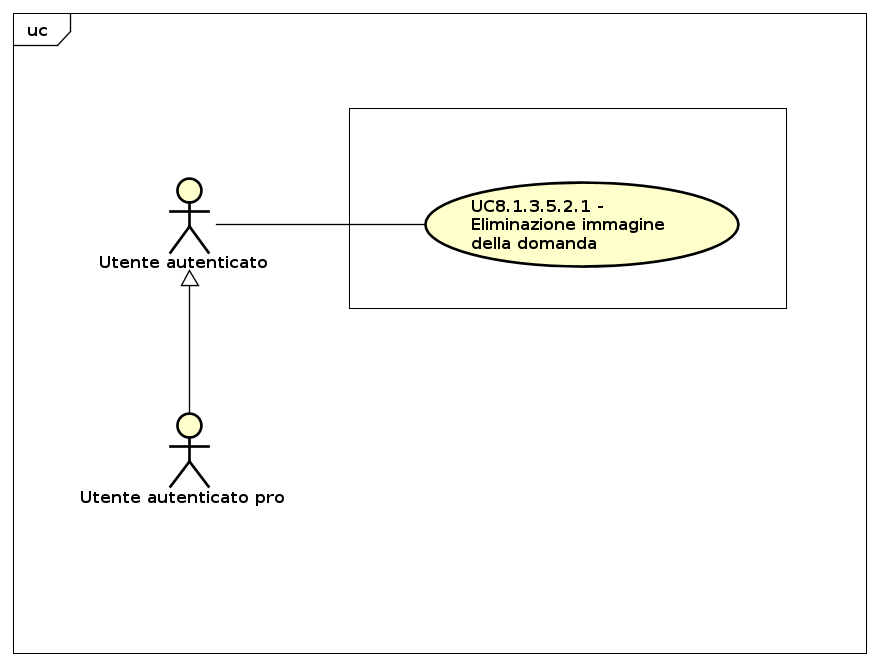
\includegraphics[scale=0.45,keepaspectratio]{UML/UC8_1_3_5_2.png}
	\caption{UC8.1.3.5.2: Inserimento immagine per testo domanda}
\end{figure}
\FloatBarrier
\begin{itemize}
	\item\textbf{Attori}: utente autenticato, utente autenticato pro;
	\item\textbf{Descrizione}: l'attore può inserire un'immagine relativa al testo della domanda;
	\item\textbf{Precondizione}: l'attore ha selezionato la funzionalità di creazione della domanda a ordinamento di immagini; 
	\item \textbf{Postcondizione}: l'attore ha inserito un'immagine relativa al testo della domanda;
	\item\textbf{Scenario principale}: 
		\begin{enumerate}
			\item L'attore può eliminare l'immagine inserita (UC8.1.3.5.2.1).
		\end{enumerate}
\end{itemize}

\subsubsection{Caso d'uso UC8.1.3.5.2.1: Eliminazione immagine per testo domanda}
\begin{itemize}
	\item\textbf{Attori}: utente autenticato, utente autenticato pro;
	\item\textbf{Descrizione}: l'attore può rimuovere l'immagine, relativa al testo della domanda, che era stata inserita precedentemente;
	\item\textbf{Precondizione}: l'attore ha inserito un immagine relativa al testo della domanda;
	\item \textbf{Postcondizione}: l'attore ha eliminato l'immagine relativa alla domanda;
	\item\textbf{Scenario principale}: l'attore rimuove l'immagine relativa alla domanda. 
\end{itemize}

\subsubsection{Caso d'uso UC8.1.3.5.3: Inserimento immagini come risposta}
\label{UC8.1.3.5.3}
\begin{figure}[h]
	\centering
	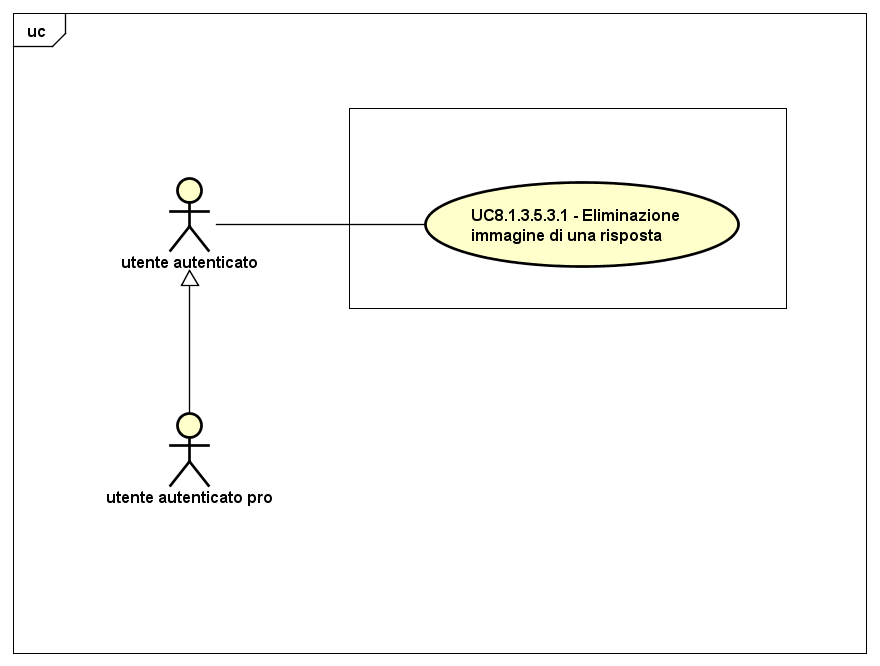
\includegraphics[scale=0.45,keepaspectratio]{UML/UC8_1_3_5_3.png}
	\caption{UC8.1.3.5.3: Inserimento immagini come risposta}
\end{figure}
\begin{itemize}
	\item\textbf{Attori}: utente autenticato, utente autenticato pro;
	\item\textbf{Descrizione}: l'attore può inserire le immagini come risposta alla domanda e indicare la soluzione di questa mettendole nell'ordine corretto;
	\item\textbf{Precondizione}: l'attore ha selezionato la funzionalità di creazione della domanda a ordinamento di immagini; 
	\item \textbf{Postcondizione}: l'attore ha inserito delle immagini come risposta alla domanda e le ha ordinate in base alla soluzione di questa;
	\item\textbf{Scenario principale}:
		\begin{enumerate}
			\item L'attore può eliminare un'immagine inserita (UC8.1.3.5.3.1).
		\end{enumerate}
\end{itemize}
\subsubsection{Caso d'uso UC8.1.3.5.3.1: Eliminazione immagine di una risposta}
\begin{itemize}
	\item\textbf{Attori}: utente autenticato, utente autenticato pro;
	\item\textbf{Descrizione}: l'attore può rimuovere un'immagine inserita come risposta;
	\item\textbf{Precondizione}: l'attore ha inserito almeno un'immagine come risposta; 
	\item \textbf{Postcondizione}: l'attore ha eliminato un'immagine relativa alla risposta;
	\item\textbf{Scenario principale}: l'attore rimuove un'immagine relativa alla risposta. 
\end{itemize}
ciao
\subsubsection{Caso d'uso UC8.1.3.7: Creazione domanda con area cliccabile nell'immagine}
\label{UC8.1.3.7}
\begin{figure}[h]
	\centering
	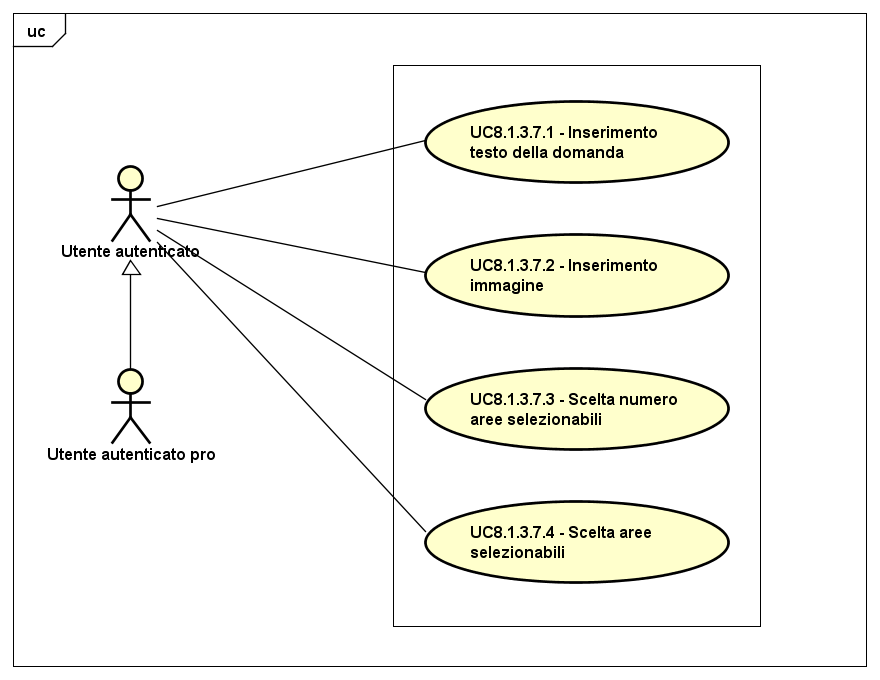
\includegraphics[scale=0.5,keepaspectratio]{UML/UC8_1_3_7.png}
	\caption{UC8.1.3.7: Creazione domanda con area cliccabile nell'immagine}
\end{figure}
\FloatBarrier
\begin{itemize}
	\item \textbf{Attori}: utente autenticato, utente autenticato pro;
	\item \textbf{Descrizione}: l'attore ha selezionato la funzionalità di creazione di una domanda la cui risposta è selezionabile all'interno di aree cliccabili in un'immagine;
	\item \textbf{Precondizione}: l'attore ha selezionato la funzionalità di creazione di una domanda con area cliccabile nell'immagine; 
	\item \textbf{Postcondizione}: l'attore han creato una domanda con area cliccabile nell'immagine;
	\item \textbf{Scenario principale}:
		\begin{enumerate}
	       	\item L'attore può inserire il testo della domanda (UC8.1.3.7.1);
	        \item L'attore può inserire una immagine relativa al testo della domanda (UC8.1.3.7.2);
		\item L'attore può scegliere quante aree saranno selezionabili all'interno dell'immagine (UC8.1.3.7.3);
		\item L'attore può scegliere quali aree saranno selezionabili all'interno dell'immagine (UC8.1.3.7.4).
	 	\end{enumerate}
\end{itemize}

\subsubsection{Caso d'uso UC8.1.3.7.1: Inserimento testo della domanda}
\begin{itemize}
	\item \textbf{Attori}: utente autenticato, utente autenticato pro;
	\item \textbf{Descrizione}: l'attore può inserire il testo della domanda che vuole creare;
	\item \textbf{Precondizione}: l'attore ha selezionato la funzionalità di creazione di una domanda con area cliccabile;
	\item \textbf{Postcondizione}: l'attore ha inserito il testo della domanda;
	\item \textbf{Scenario principale}: l'attore inserisce il testo della domanda. 
\end{itemize}

\subsubsection{Caso d'uso UC8.1.3.7.2: Inserimento immagine}
\begin{itemize}
	\item \textbf{Attori}: utente autenticato, utente autenticato pro;
	\item \textbf{Descrizione}: l'attore può inserire un'immagine relativa al testo della domanda;
	\item \textbf{Precondizione}: l'attore ha selezionato la funzionalità di creazione di una domanda con area cliccabile; 
	\item \textbf{Postcondizione}: l'attore ha inserito un'immagine relativa al testo della domanda;
	\textbf{Scenario principale}: 
			\begin{enumerate}
				\item L'attore può eliminare l'immagine inserita (UC8.1.3.7.2.1).	
			\end{enumerate}						
	\end{itemize}

\subsubsection{Caso d'uso UC8.1.3.7.3: Scelta numero aree selezionabili}
\begin{itemize}
	\item \textbf{Attori}: utente autenticato, utente autenticato pro;
	\item \textbf{Descrizione}: l'attore può scegliere il numero di aree selezionabili all'interno dell'immagine;
	\item \textbf{Precondizione}: l'attore ha selezionato la funzionalità di creazione di una domanda con area cliccabile; 
	\item \textbf{Postcondizione}: l'attore ha scelto il numero di aree selezionabili all'interno dell'immagine;
	\item \textbf{Scenario principale}: l'attore sceglie il numero di aree selezionabili all'interno dell'immagine. 	
\end{itemize}

\subsubsection{Caso d'uso UC8.1.3.7.4: Scelta aree selezionabili}
\begin{itemize}
	\item \textbf{Attori}: utente autenticato, utente autenticato pro;
	\item \textbf{Descrizione}: l'attore ha la possibilità di scegliere dove inserire le aree selezionabili all'interno dell'immagine;
	\item \textbf{Precondizione}: l'attore ha selezionato la funzionalità di creazione di una domanda con area cliccabile; 
	\item \textbf{Postcondizione}: l'attore ha scelto dove inserire le aree selezionabili all'interno dell'immagine;
	\item \textbf{Scenario principale}: l'attore sceglie dove inserire le aree selezionabili all'interno dell'immagine. 	
\end{itemize}




	\subsubsection{Caso d'uso UC8.1.4: Conferma creazione}
	\begin{itemize}
		\item
			\textbf{Attori}: utente autenticato, utente autenticato pro;
		\item
			\textbf{Descrizione}: l'attore può confermare la creazione della domanda;
		\item		
			\textbf{Precondizione}: l'attore ha finito di creare una domanda tramite un wizard;
		\item
			\textbf{Postcondizione}: l'attore ha creato una domanda;
		\item
			\textbf{Scenario principale}: l'attore conferma la creazione della domanda;		
		\item
	 		\textbf{Scenari alternativi}: l'attore annulla la creazione della domanda.
					
	\end{itemize}	
	
	\subsubsection{Caso d'uso UC8.1.5: Visualizzazione errore creazione domanda}
	\begin{itemize}
		\item
			\textbf{Attori}: utente autenticato, utente autenticato pro;
		\item
			\textbf{Descrizione}: l'attore può visualizzare un messaggio d'errore nel caso si fossero verificati uno o più scenari alternativi durante la creazione della domanda;
		\item		
			\textbf{Precondizione}: il sistema ha ricevuto dei dati errati per la creazione della domanda;
		\item
			\textbf{Postcondizione}: il sistema mostra un messaggio d'errore;
		\item
			\textbf{Scenario principale}: l'attore visualizza un messaggio d'errore;	
	\end{itemize}	


	\subsubsection{Caso d'uso UC8.2: Modifica domanda esistente}
	\label{UC8.2}
	\begin{figure}[h]
		\centering
			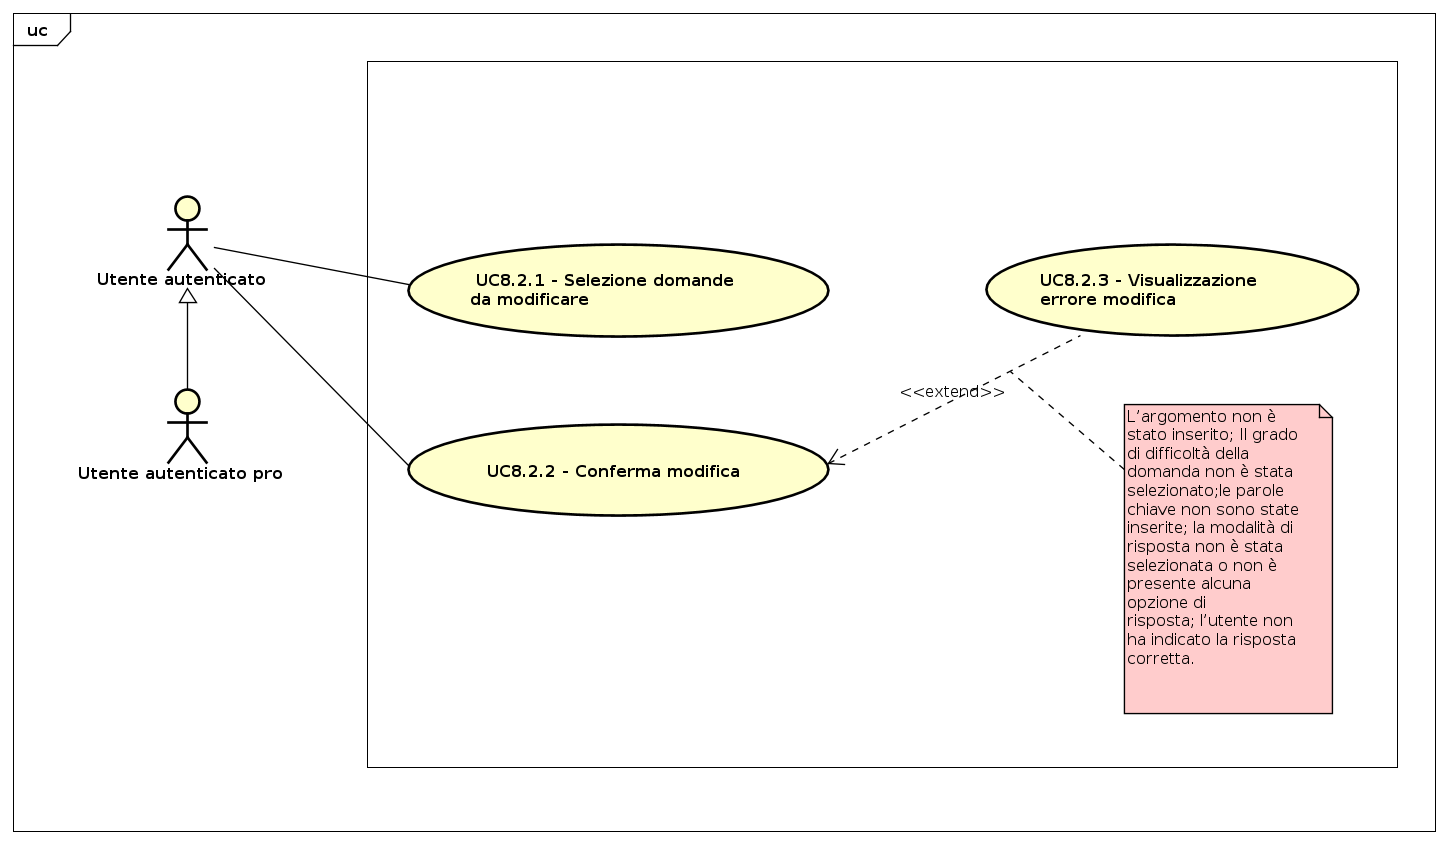
\includegraphics[scale=0.45,keepaspectratio]{UML/UC8_2.png}
		\caption{UC8.2: Modifica domanda esistente}
	\end{figure}
	\FloatBarrier
	\begin{itemize}
		\item
			\textbf{Attori}: utente autenticato, utente autenticato pro;
		\item		
			\textbf{Descrizione}: l'attore può modificare una domanda che aveva creato precedentemente;
		\item
			\textbf{Precondizione}: l'attore ha selezionato la funzionalità di modifica domanda;
		\item
			\textbf{Postcondizione}: l'attore modifica una domanda;
		\item
			\textbf{Scenario principale}:
				\begin{enumerate}
					\item
						L'attore può selezionare la domanda da modificare (UC8.2.1);
				\end{enumerate}
	       		
	 	\item
			\textbf{Estensioni}: l'attore visualizza un messaggio d'errore relativo alla modifica della domanda (UC8.2.3);
	 	\item
	 		\textbf{Scenari alternativi}:
				\begin{itemize}
					\item 	
						L'argomento non è stato inserito;
					\item
						Le parole chiave non sono state inserite;
					\item
						Non tutti i campi obbligatori sono stati inseriti; 
					\item
						Non è stata indicata la risposta corretta.	
				\end{itemize}
	\end{itemize}
	
		\subsubsection{Caso d'uso UC8.2.1: Selezione domande da modificare}
		\label{UC8.2.1}
		\begin{figure}[h]
			\centering
			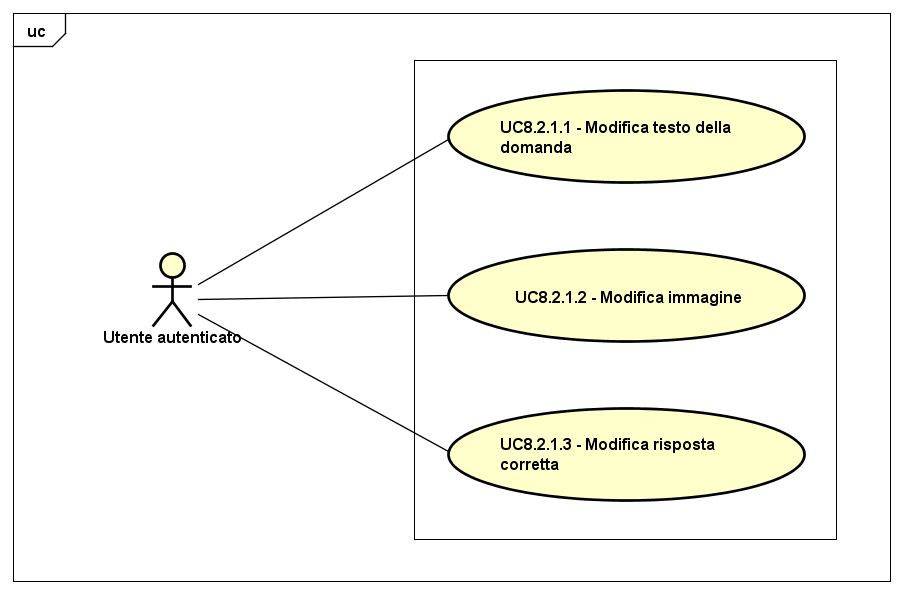
\includegraphics[scale=0.5,keepaspectratio]{UML/UC8_2_1.png}
			\caption{Caso d'uso UC8.2.1: Selezione domande da modificare}
		\end{figure}
		\FloatBarrier
		\begin{itemize}
			\item \textbf{Attori}: utente autenticato, utente autenticato pro;
			\item \textbf{Descrizione}: l'attore può selezionare la domanda da modificare;
			\item \textbf{Precondizione}: l'attore ha selezionato la funzionalità di modifica domanda;
			\item \textbf{Postcondizione}: l'attore ha selezionato la domanda da modificare; 
			\item \textbf{Scenario principale}: 
					\begin{enumerate}
					\item
					L'attore può richiamare il wizard per modificare una domanda vero/falso (UC8.2.1.1);
					\item
					L'attore può richiamare il wizard per modificare una domanda a risposta multipla (UC8.2.1.2);
					\item
					L'attore può richiamare il wizard per modificare un esercizio a riempimento di spazi vuoti (UC8.2.1.3);
					\item
					L'attore può richiamare il wizard per modificare una domanda di collegamento (UC8.2.1.4);
					\item
					L'attore può richiamare il wizard per modificare una domanda a ordinamento di immagini (UC8.2.1.5);
					\item
					L'attore può richiamare il wizard per modificare una domanda a ordinamento di stringhe (UC8.2.1.6);
					\item
					L'attore può richiamare il wizard per modificare una domanda con area cliccabile nell'immagine (UC8.2.1.7).
	 			\end{enumerate}
			
		\end{itemize}

	%inclusione file latex wizard
\subsubsection{Caso d'uso UC8.2.1.1: Modifica domanda vero/falso}
	\label{UC8.2.1.1}
	\begin{figure}[h]
		\centering
			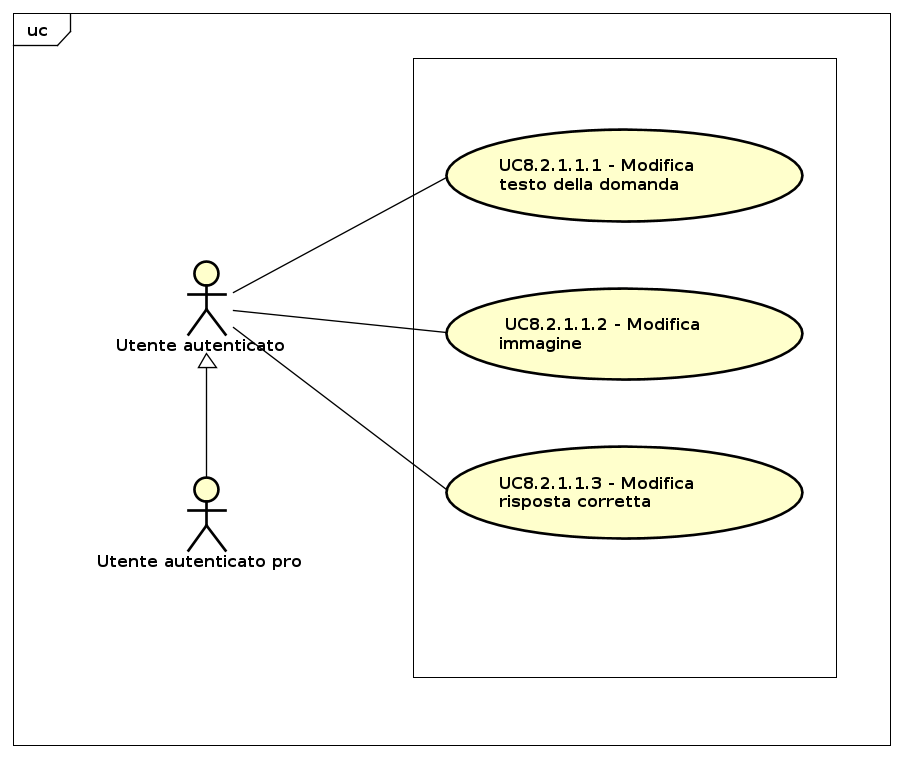
\includegraphics[scale=0.45,keepaspectratio]{UML/UC8_2_1_1.png}
		\caption{UC8.2.1.1: Modifica domanda vero/falso}
	\end{figure}
	\FloatBarrier
	\begin{itemize}
		\item
			\textbf{Attori}: utente autenticato, utente autenticato pro;
		\item		
			\textbf{Descrizione}: l'attore può utilizzare la procedura guidata per la modifica di una domanda vero/falso;
		\item
			\textbf{Precondizione}: l'attore ha selezionato la funzionalità di modifica di una domanda \\vero/falso; 
		\item
			\textbf{Postcondizione}: l'attore ha modificato una domanda vero/falso;
		\item
			\textbf{Scenario principale}:
	       		\begin{enumerate}
	       			\item
	       			L'attore può modificare il testo della domanda (UC8.2.1.1.1);
	       			\item
	       			L'attore può modificare l'immagine relativa al testo della domanda (UC8.2.1.1.2);
					\item
					L'attore può modificare la risposta corretta (UC8.2.1.1.3).
	 			\end{enumerate}
	\end{itemize}
	
\subsubsection{Caso d'uso UC8.2.1.1.1: Modifica testo della domanda}
	\begin{itemize}
		\item
			\textbf{Attori}: utente autenticato, utente autenticato pro;
		\item		
			\textbf{Descrizione}: l'attore può modificare il testo della domanda;
		\item
			\textbf{Precondizione}: l'attore ha selezionato la funzionalità di modifica di una domanda \\vero/falso; 
		\item
			\textbf{Postcondizione}: l'attore ha modificato il testo della domanda;
		\item
			\textbf{Scenario principale}: l'attore modifica il testo della domanda. 
	\end{itemize}
	
\subsubsection{Caso d'uso UC8.2.1.1.2: Modifica immagine}
	\begin{itemize}
		\item
			\textbf{Attori}: utente autenticato, utente autenticato pro;
		\item		
			\textbf{Descrizione}: l'attore può modificare l'immagine relativa al testo della domanda;
		\item
			\textbf{Precondizione}: l'attore ha selezionato la funzionalità di modifica di una domanda \\vero/falso; 
		\item
			\textbf{Postcondizione}: l'attore ha modificato l'immagine relativa al testo della domanda;
		\item
			\textbf{Scenario principale}: l'attore modifica l'immagine relativa al testo della domanda. 	
	\end{itemize}
	
\subsubsection{Caso d'uso UC8.2.1.1.3: Modifica risposta corretta}
	\begin{itemize}
		\item
			\textbf{Attori}: utente autenticato, utente autenticato pro;
		\item		
			\textbf{Descrizione}: l'attore può modificare la selezione della risposta corretta;
		\item
			\textbf{Precondizione}: l'attore ha selezionato la funzionalità di modifica di una domanda \\vero/falso; 
		\item
			\textbf{Postcondizione}: l'attore ha modificato la selezione della risposta corretta;
		\item
			\textbf{Scenario principale}: l'attore modifica la selezione della risposta corretta.	 			
	\end{itemize}
	

\subsubsection{Caso d'uso UC8.2.1.2: Modifica domanda a risposta multipla}
	\label{UC8.2.1.2}
	\begin{figure}[h]
		\centering
			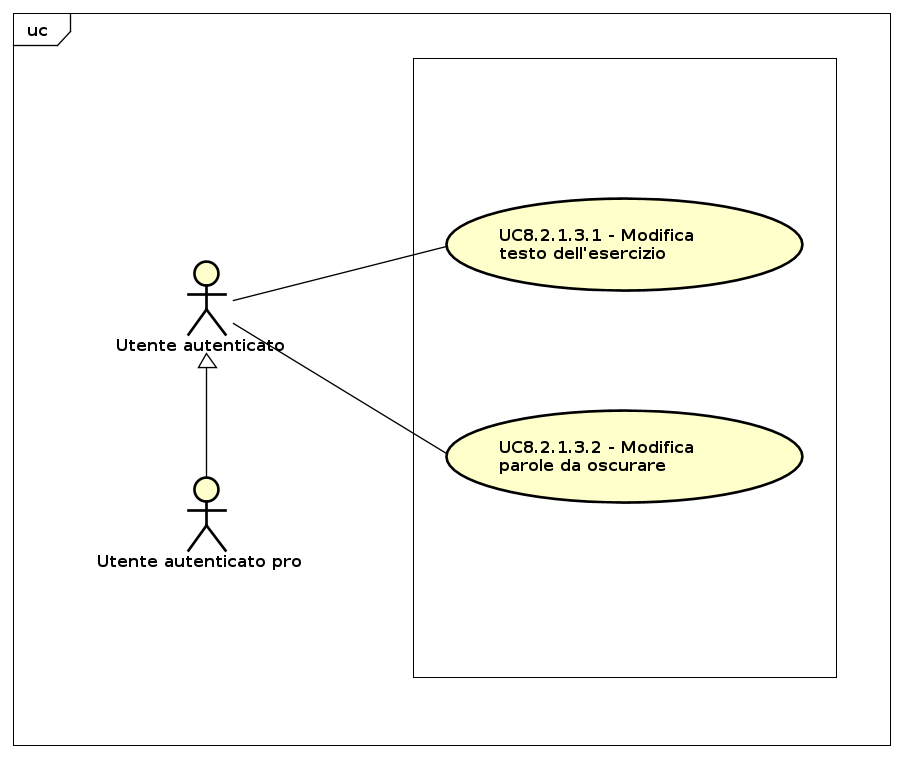
\includegraphics[scale=0.45,keepaspectratio]{UML/UC8_2_1_2.png}
		\caption{UC8.2.1.2: Modifica domanda a risposta multipla}
	\end{figure}
	\FloatBarrier
	\begin{itemize}
		\item
			\textbf{Attori}: utente autenticato, utente autenticato pro;
		\item		
			\textbf{Descrizione}: l'attore può utilizzare la procedura guidata per la modifica di una domanda a risposta multipla;
		\item
			\textbf{Precondizione}: l'attore ha selezionato la funzionalità di modifica di una domanda a risposta multipla; 
		\item
			\textbf{Postcondizione}: l'attore ha modificato una domanda a risposta multipla;
		\item
			\textbf{Scenario principale}:
	       		\begin{enumerate}
	       			\item
	       			L'attore può modificare il testo della domanda (UC8.2.1.2.1);
	       			\item
	       			L'attore può modificare l'immagine relativa al testo della domanda (UC8.2.1.2.2);
	       			\item
	       			L'attore può modificare le opzioni di risposta (UC8.2.1.2.3);
					\item
					L'attore può modificare la/le risposte corrette (UC8.2.1.2.4).
	 			\end{enumerate}
	\end{itemize}

\subsubsection{Caso d'uso UC8.2.1.2.1: Modifica testo della domanda}
	\begin{itemize}
		\item
			\textbf{Attori}: utente autenticato, utente autenticato pro;
		\item		
			\textbf{Descrizione}: l'attore può modificare il testo della domanda;
		\item
			\textbf{Precondizione}: l'attore ha selezionato la funzionalità di modifica di una domanda a risposta multipla;
		\item
			\textbf{Postcondizione}: l'attore ha modificato il testo della domanda;
		\item
			\textbf{Scenario principale}: l'attore modifica il testo della domanda. 
	 			
	\end{itemize}
	
\subsubsection{Caso d'uso UC8.2.1.2.2: Modifica immagine}
	\begin{itemize}
		\item
			\textbf{Attori}: utente autenticato, utente autenticato pro;
		\item		
			\textbf{Descrizione}: l'attore può modificare l'immagine relativa al testo della domanda;
		\item
			\textbf{Precondizione}: l'attore ha selezionato la funzionalità di modifica di una domanda a risposta multipla;
		\item
			\textbf{Postcondizione}: l'attore ha modificato l'immagine relativa al testo della domanda;
		\item
			\textbf{Scenario principale}: l'attore modifica l'immagine relativa al testo della domanda. 	
	\end{itemize}
	
	
\subsubsection{Caso d'uso UC8.2.1.2.3: Modifica opzioni di risposta}
	\label{UC8.2.1.2.3}
	\begin{figure}[h]
		\centering
			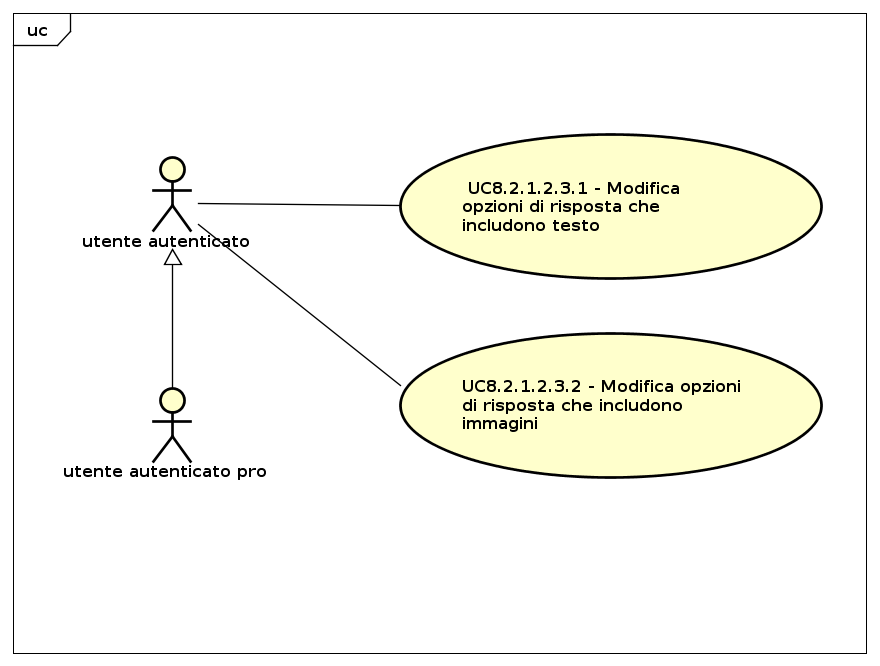
\includegraphics[scale=0.45,keepaspectratio]{UML/UC8_2_1_2_3.png}
		\caption{UC8.2.1.2.3: Modifica opzioni di risposta}
	\end{figure}
	\FloatBarrier
	\begin{itemize}
		\item
			\textbf{Attori}: utente autenticato, utente autenticato pro;
		\item		
			\textbf{Descrizione}: l'attore può modificare le opzioni di risposta;
		\item
			\textbf{Precondizione}: l'attore ha selezionato la funzionalità di modifica di una domanda a risposta multipla;
		\item
			\textbf{Postcondizione}: l'attore ha modificato le opzioni di risposta;
		\item
			\textbf{Scenario principale}:
	       		\begin{enumerate}
	       			\item
	       			L'attore può modificare opzioni di risposta che includono testo (UC8.2.1.2.3.1);
					\item
					L'attore può modificare opzioni di risposta che includono immagini (UC8.2.1.2.3.2).
	 			\end{enumerate}
	\end{itemize}	
	
\subsubsection{Caso d'uso UC8.2.1.2.3.1: Modifica opzioni di risposta che includono testo}
	\begin{itemize}
		\item
			\textbf{Attori}: utente autenticato, utente autenticato pro;
		\item		
			\textbf{Descrizione}: l'attore può modificare le opzioni di risposta che includono testo;
		\item
			\textbf{Precondizione}: l'attore ha selezionato la funzionalità di modifica di una domanda a risposta multipla con opzioni di risposta che includono testo; 
		\item
			\textbf{Postcondizione}: l'attore ha modificato le opzioni di risposta che includono testo;
		\item
			\textbf{Scenario principale}: l'attore modifica le opzioni di risposta che includono testo. 			
	\end{itemize}	
	
\subsubsection{Caso d'uso UC8.2.1.2.3.2: Modifica opzioni di risposta che includono immagini}
	\begin{itemize}
		\item
			\textbf{Attori}: utente autenticato, utente autenticato pro;
		\item		
			\textbf{Descrizione}: l'attore può modificare le opzioni di risposta che includono immagini;
		\item
			\textbf{Precondizione}: l'attore ha selezionato la funzionalità di modifica di una domanda a risposta multipla con opzioni di risposta che includono immagini; 
		\item
			\textbf{Postcondizione}: l'attore ha modificato le opzioni di risposta che includono immagini;
		\item
			\textbf{Scenario principale}: l'attore modifica le opzioni di risposta che includono immagini. 			
	\end{itemize}
	
\subsubsection{Caso d'uso UC8.2.1.2.4: Modifica risposte corrette}
	\begin{itemize}
		\item
			\textbf{Attori}: utente autenticato, utente autenticato pro;
		\item		
			\textbf{Descrizione}: l'attore può modificare la selezione delle risposte corrette;
		\item
			\textbf{Precondizione}: l'attore ha selezionato la funzionalità di modifica di una domanda a risposta multipla;
		\item
			\textbf{Postcondizione}: l'attore ha modificato la selezione delle risposte corrette;
		\item
			\textbf{Scenario principale}: l'attore modifica la selezione delle risposte corrette. 			
	\end{itemize}

\subsubsection{Caso d'uso UC8.2.1.3: Modifica esercizi di riempimento degli spazi vuoti}
	\label{UC8.2.1.3}
	\begin{figure}[h]
		\centering
			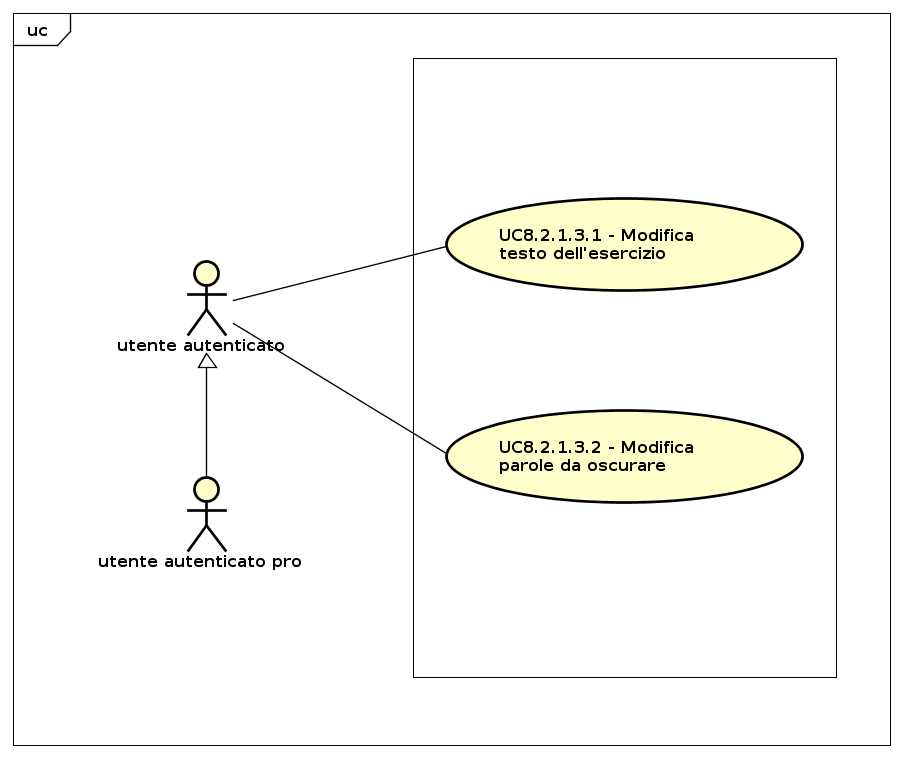
\includegraphics[scale=0.45,keepaspectratio]{UML/UC8_2_1_3.png}
		\caption{UC8.2.1.3: Modifica esercizi di riempimento degli spazi vuoti}
	\end{figure}
	\FloatBarrier
	\begin{itemize}
		\item
			\textbf{Attori}: utente autenticato, utente autenticato pro;
		\item		
			\textbf{Descrizione}: l'attore può utilizzare la procedura guidata per la modifica di un esercizio di riempimento degli spazi vuoti;
		\item
			\textbf{Precondizione}: l'attore ha selezionato la funzionalità di modifica di un esercizio di riempimento degli spazi vuoti; 
		\item
			\textbf{Postcondizione}: l'attore ha modificato un esercizio di riempimento degli spazi vuoti;
		\item
			\textbf{Scenario principale}:
	       		\begin{enumerate}
	       			\item
	       			L'attore può modificare il testo dell'esercizio (UC8.2.1.3.1);
	       			\item
	       			L'attore può modificare le parole che saranno sostituite con degli spazi vuoti dal sistema (UC8.2.1.3.2).
	 			\end{enumerate}
	\end{itemize}
	
\subsubsection{Caso d'uso UC8.2.1.3.1: Modifica testo dell'esercizio}
	\begin{itemize}
		\item
			\textbf{Attori}: utente autenticato, utente autenticato pro;
		\item		
			\textbf{Descrizione}: l'attore può modificare il testo dell'esercizio;
		\item
			\textbf{Precondizione}: l'attore ha selezionato la funzionalità di modifica di un esercizio di riempimento degli spazi vuoti; 
		\item
			\textbf{Postcondizione}: l'attore ha modificato il testo dell'esercizio;
		\item
			\textbf{Scenario principale}: l'attore modifica il testo dell'esercizio.
	\end{itemize}


\subsubsection{Caso d'uso UC8.2.1.3.2: Modifica parole da oscurare}
	\begin{itemize}
		\item
			\textbf{Attori}: utente autenticato, utente autenticato pro;
		\item		
			\textbf{Descrizione}: l'attore può modificare le parole che saranno sostituite con degli spazi vuoti;
		\item
			\textbf{Precondizione}: l'attore ha selezionato la funzionalità di modifica di un esercizio di riempimento degli spazi vuoti; 
		\item
			\textbf{Postcondizione}: l'attore ha modificato le parole che saranno sostituite con degli spazi vuoti;
		\item
			\textbf{Scenario principale}: l'attore modifica le parole che verranno oscurate dal sistema.
	\end{itemize}

\subsubsection{Caso d'uso UC8.2.1.4: Modifica domanda di collegamento}
\label{UC8.2.1.4}
\begin{figure}[h]
	\centering
	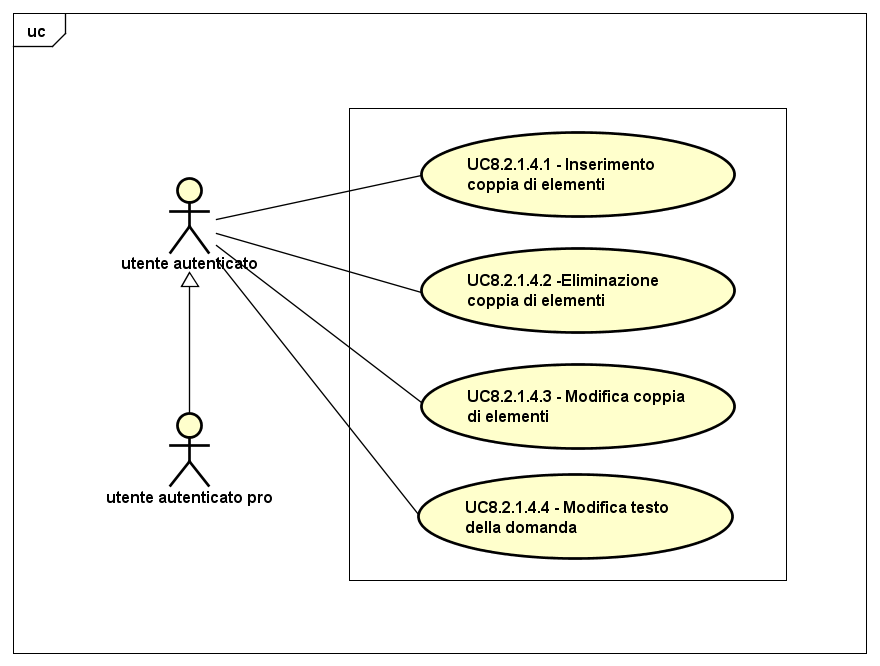
\includegraphics[scale=0.5,keepaspectratio]{UML/UC8_2_1_4.png}
	\caption{Caso d'uso UC8.2.1.4: Modifica domanda di collegamento}
\end{figure}
\FloatBarrier
\begin{itemize}
	\item \textbf{Attori}: \uau, \uaupro;
	\item \textbf{Descrizione}: l'attore può utilizzare la procedura guidata per la modifica di una domanda di collegamento; 
	\item \textbf{Precondizione}: l'attore ha selezionato la funzionalità di modifica di una domanda di collegamento; 
	\item \textbf{Postcondizione}: l'attore ha modificato una domanda di collegamento;
	\item \textbf{Scenario principale}: 
	\begin{enumerate}
			\item L'attore può modificare il testo della domanda (UC8.2.1.4.1);
			\item L'attore può inserire una coppia di elementi (UC8.2.1.4.2);
			\item L'attore può eliminare una coppia di elementi inserita (UC8.2.1.4.3);
			\item L'attore può modificare una coppia di elementi inserita (UC8.2.1.4.4).
		\end{enumerate}
	\item \textbf{Scenari alternativi}: se non ci sono almeno due coppie presenti nella lista delle coppie l'attore deve inserire una nuova coppia di elementi.
\end{itemize}

	\subsubsection{Caso d'uso UC8.2.1.4.1: Modifica testo della domanda}
	\label{UC8.2.1.4.1}
	\begin{itemize}
		\item
		\textbf{Attori}: \uau, \uaupro;
		\item		
		\textbf{Descrizione}: l'attore può modificare il testo della domanda;
		\item
		\textbf{Precondizione}: l'attore ha selezionato la funzionalità di modifica di una domanda di collegamento; 
		\item
		\textbf{Postcondizione}: l'attore ha modificato il testo della domanda;
		\item
		\textbf{Scenario principale}: l'attore modifica il testo della domanda.	
	\end{itemize}

	\subsubsection{Caso d'uso UC8.2.1.4.2: Inserimento coppia di elementi}
	\label{UC8.2.1.4.2}
	\begin{figure}[h]
		\centering
		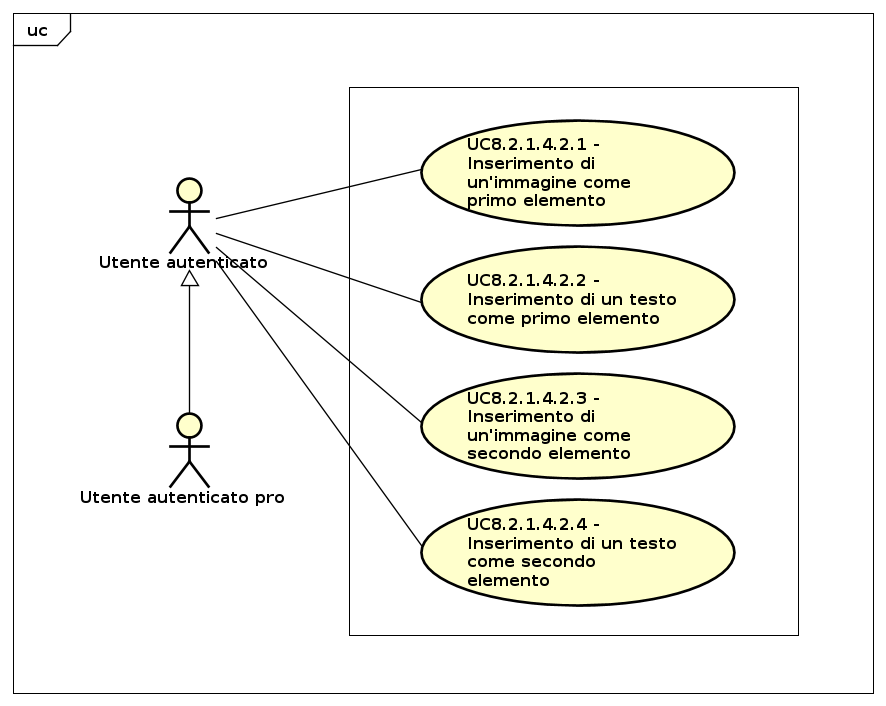
\includegraphics[scale=0.5,keepaspectratio]{UML/UC8_2_1_4_2.png}
		\caption{Caso d'uso UC8.2.1.4.2: Inserimento coppia di elementi}
	\end{figure}
	\FloatBarrier
	\begin{itemize}
		\item \textbf{Attori}: \uau, \uaupro;
		\item \textbf{Descrizione}: l'attore può inserire una coppia di elementi, sia immagini che testo o combinazioni di questi, che siano correlati tra loro in modo da indicare la soluzione della domanda. 
		\item \textbf{Precondizione}: l'attore ha selezionato la funzionalità di modifica di una domanda di collegamento;
		\item \textbf{Postcondizione}: l'attore ha inserito una coppia di elementi nella lista di coppie di elementi; 
		\item \textbf{Scenario principale}: 
		\begin{enumerate}
			\item L'attore inserisce come primo elemento un'immagine (UC8.2.1.4.2.1);
			\item L'attore inserisce come primo elemento un testo (UC8.2.1.4.2.2);
			\item L'attore inserisce come secondo elemento un'immagine (UC8.2.1.4.2.3);
			\item L'attore inserisce come secondo elemento un testo (UC8.2.1.4.2.4).	
		\end{enumerate}
	\end{itemize}
	
		\subsubsection{Caso d'uso UC8.2.1.4.2.1: Inserimento di un'immagine come primo elemento}
		\label{UC8.2.1.4.2.1}
		\begin{itemize}
			\item \textbf{Attori}: \uau, \uaupro;
			\item \textbf{Descrizione}: l'attore può inserire come primo elemento della coppia un'immagine;
			\item \textbf{Precondizione}: l'attore sta selezionando una coppia di elementi;
			\item \textbf{Postcondizione}: l'attore ha inserito come primo elemento un'immagine;
			\item \textbf{Scenario principale}: l'attore carica un'immagine come primo elemento della coppia.
		\end{itemize}
		
		\subsubsection{Caso d'uso UC8.2.1.4.2.2: Inserimento di un testo come primo elemento}
		\label{UC8.2.1.4.2.2}
		\begin{itemize}
			\item \textbf{Attori}: \uau, \uaupro;
			\item \textbf{Descrizione}: l'attore può inserire come primo elemento della coppia un testo;
			\item \textbf{Precondizione}: l'attore sta selezionando una coppia di elementi;
			\item \textbf{Postcondizione}: l'attore ha inserito come primo elemento un testo;
			\item \textbf{Scenario principale}: l'attore inserisce del testo come primo elemento della coppia.
		\end{itemize}
		
			\subsubsection{Caso d'uso UC8.2.1.4.2.3: Inserimento di un'immagine come secondo elemento}
		\label{UC8.2.1.4.2.3}
		\begin{itemize}
			\item \textbf{Attori}: \uau, \uaupro;
			\item \textbf{Descrizione}: l'attore può inserire come secondo elemento della coppia un'immagine;
			\item \textbf{Precondizione}: l'attore sta selezionando una coppia di elementi;
			\item \textbf{Postcondizione}: l'attore ha inserito come secondo elemento un'immagine;
			\item \textbf{Scenario principale}: l'attore carica un'immagine come secondo elemento della coppia.
		\end{itemize}
		
		\subsubsection{Caso d'uso UC8.2.1.4.2.4: Inserimento di un testo come secondo elemento}
		\label{UC8.2.1.4.2.4}
		\begin{itemize}
			\item \textbf{Attori}: \uau, \uaupro;
			\item \textbf{Descrizione}: l'attore può inserire come secondo elemento della coppia un testo;
			\item \textbf{Precondizione}: l'attore sta selezionando una coppia di elementi;
			\item \textbf{Postcondizione}: l'attore ha inserito come secondo elemento un testo;
			\item \textbf{Scenario principale}: l'attore inserisce del testo come secondo elemento della coppia.
		\end{itemize}
	
	\subsubsection{Caso d'uso UC8.2.1.4.3: Eliminazione coppia di elementi}
	\label{UC8.2.1.4.3}
	\begin{figure}[h]
		\centering
		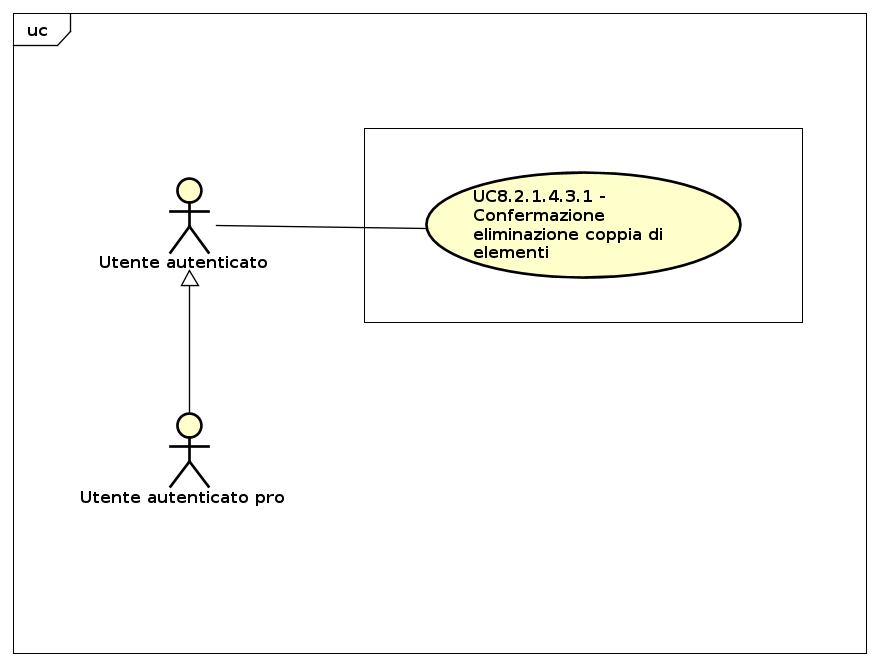
\includegraphics[scale=0.5,keepaspectratio]{UML/UC8_2_1_4_3.png}
		\caption{Caso d'uso UC8.2.1.4.3: Eliminazione coppia di elementi}
	\end{figure}
	\FloatBarrier
	\begin{itemize}
		\item \textbf{Attori}: \uau, \uaupro;
		\item \textbf{Descrizione}: l'attore può rimuovere una coppia di elementi dalla lista di coppie di elementi;
		\item \textbf{Precondizione}: l'attore ha inserito almeno una coppia di elementi;
		\item \textbf{Postcondizione}: l'attore ha eliminato una coppia di elementi dalla lista delle coppie di elementi;
		\item \textbf{Scenario principale}: 
		\begin{enumerate}
		\item L'attore può confermare l'eliminazione di una coppia di elementi (UC8.2.1.4.3.1).
		\end{enumerate}	
		\item \textbf{Scenari alternativi}: l'attore annulla l'operazione tornando alla schermata precedente.
	\end{itemize}

		\subsubsection{Caso d'uso UC8.2.1.4.3.1: Conferma eliminazione coppia di elementi}
		\label{UC8.2.1.4.3.1}
		\begin{itemize}
			\item \textbf{Attori}: \uau, \uaupro;
			\item \textbf{Descrizione}: l'attore può confermare la rimozione di una coppia di elementi;
			\item \textbf{Precondizione}: l'attore ha eliminato una coppia di elementi dalla lista delle coppie di elementi;
			\item \textbf{Postcondizione}: l'attore ha confermato l'eliminazione della coppia di elementi;
			\item \textbf{Scenario principale}: l'attore conferma la rimozione della coppia di elementi.
		\end{itemize}

	\subsubsection{Caso d'uso UC8.2.1.4.4: Modifica coppia di elementi}
	\label{UC8.2.1.4.4}
	\begin{figure}[h]
		\centering
		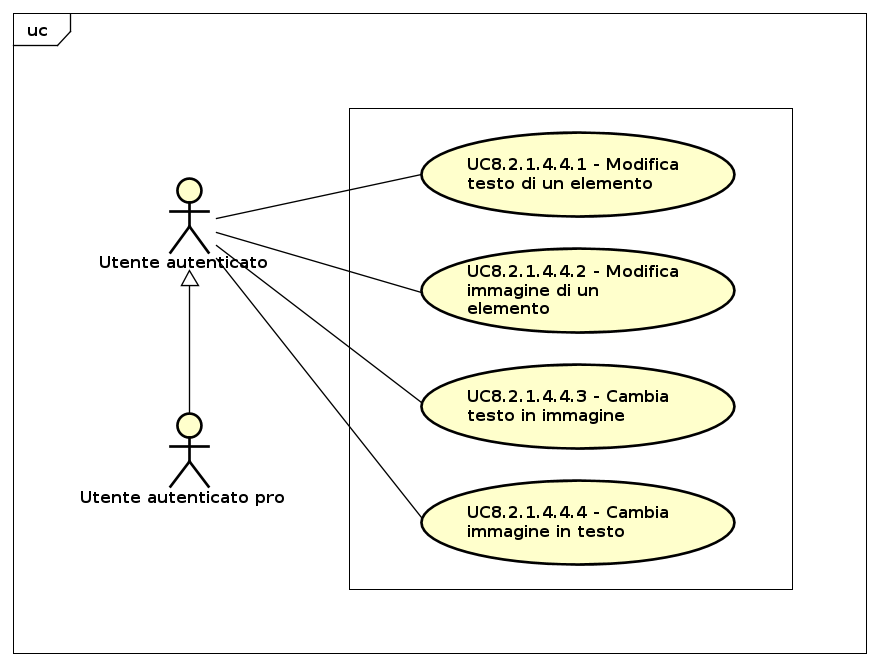
\includegraphics[scale=0.5,keepaspectratio]{UML/UC8_2_1_4_4.png}
		\caption{Caso d'uso UC8.2.1.4.4: Modifica coppia di elementi}
	\end{figure}
	\FloatBarrier
	\begin{itemize}
		\item \textbf{Attori}: \uau, \uaupro;
		\item \textbf{Descrizione}: l'attore può modificare una coppia di elementi presente nella lista di coppie di elementi;
		\item \textbf{Precondizione}: l'attore ha inserito almeno una coppia di elementi;
		\item \textbf{Postcondizione}: l'attore ha modificato una coppia di elementi presente nella lista di coppie di elementi; 
		\item \textbf{Scenario principale}: 
		\begin{enumerate}
			\item L'attore può modificare un elemento cambiandone il testo (UC8.2.1.4.4.1);
			\item L'attore può modificare un elemento cambiandone l'immagine (UC8.2.1.4.4.2);
			\item L'attore può modificare un elemento facendolo passare da testo ad immagine (UC8.2.1.4.4.3);
			\item L'attore può modificare un elemento facendolo passare da immagine a testo (UC8.2.1.4.4.4).	
		\end{enumerate}
	\end{itemize}
	
		\subsubsection{Caso d'uso UC8.2.1.4.4.1: Modifica testo di un elemento}
		\label{UC8.2.1.4.4.1}
		\begin{itemize}
			\item \textbf{Attori}: \uau, \uaupro;
			\item \textbf{Descrizione}: l'attore può modificare il testo di un elemento;
			\item \textbf{Precondizione}: l'attore sta modificando una coppia di elementi presente nella lista di coppie di elementi; 
			\item \textbf{Postcondizione}: l'attore ha modificato il testo di un elemento;
			\item \textbf{Scenario principale}: l'attore modifica il testo di un elemento.  
		\end{itemize}
		
		\subsubsection{Caso d'uso UC8.2.1.4.4.2: Modifica immagine di un elemento}
		\label{UC8.2.1.4.4.2}
		\begin{itemize}
			\item \textbf{Attori}: \uau, \uaupro;
			\item \textbf{Descrizione}: l'attore può caricare un'altra immagine per un elemento;
			\item \textbf{Precondizione}: l'attore sta modificando una coppia di elementi presente nella lista di coppie di elementi; 
			\item \textbf{Postcondizione}: l'attore ha inserito un'altra immagine per un elemento;
			\item \textbf{Scenario principale}: l'attore carica un'altra immagine per un elemento.
		\end{itemize}
		
		\subsubsection{Caso d'uso UC8.2.1.4.4.3: Cambia testo in immagine}
		\label{UC8.2.1.4.4.3}
		\begin{itemize}
			\item \textbf{Attori}: \uau, \uaupro;
			\item \textbf{Descrizione}: l'attore può modificare un elemento facendolo diventare un'immagine al posto di un testo;
			\item \textbf{Precondizione}: l'attore sta modificando una coppia di elementi presente nella lista di coppie di elementi; 
			\item \textbf{Postcondizione}: l'attore ha fatto diventare un'immagine un elemento che prima era un testo;
			\item \textbf{Scenario principale}: l'attore inserisce un'immagine come modifica dell'elemento.  
		\end{itemize}
		
		\subsubsection{Caso d'uso UC8.2.1.4.4.4: Cambia immagine in testo}
		\label{UC8.2.1.4.4.4}
		\begin{itemize}
			\item \textbf{Attori}: \uau, \uaupro;
			\item \textbf{Descrizione}: l'attore può modificare un elemento facendolo diventare un testo al posto di un'immagine;
			\item \textbf{Precondizione}: l'attore sta modificando una coppia di elementi presente nella lista di coppie di elementi; 
			\item \textbf{Postcondizione}: l'attore ha fatto diventare un testo un elemento che prima era un'immagine;
			\item \textbf{Scenario principale}: l'attore inserisce del testo come modifica dell'elemento.  
		\end{itemize}
\subsubsection{Caso d'uso UC8.2.1.5: Modifica domanda a ordinamento di immagini}
\label{UC8.2.1.5}
	\begin{figure}[h]
		\centering
			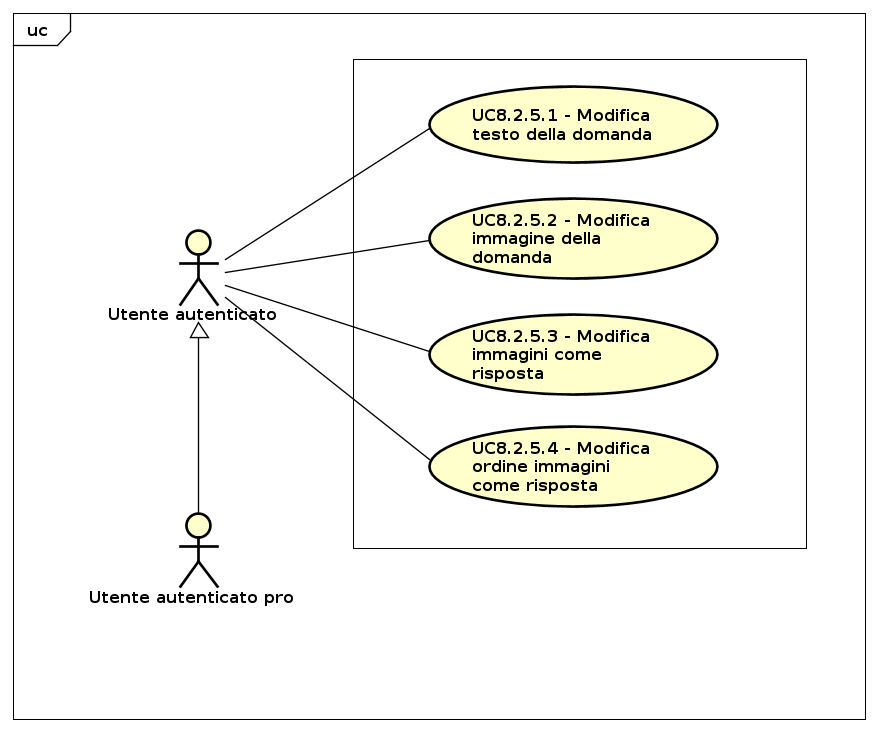
\includegraphics[scale=0.45,keepaspectratio]{UML/UC8_2_1_5.png}
		\caption{UC8.2.1.5: Modifica domanda a ordinamento di immagini}
	\end{figure}
\begin{itemize}
	\item\textbf{Attori}: utente autenticato, utente autenticato pro;
	\item\textbf{Descrizione}: l'attore può utilizzare la procedura guidata per la modifica di una domanda a ordinamento di immagini;
	\item\textbf{Precondizione}: l'attore ha selezionato la funzionalità di modifica di una domanda a ordinamento di immagini;
	\item \textbf{Postcondizione}: l'attore ha modificato una domanda a ordinamento di immagini;
	\item\textbf{Scenario principale}: 
	\begin{itemize}
		\item L'attore può modificare il testo della domanda (UC8.2.1.5.1);
		\item L'attore può modifica l'immagine relativa al testo della domanda (UC8.2.1.5.2);
		\item L'attore può modificare le immagini della sequenza che costituirà la risposta (UC8.2.1.5.3);
		\item L'attore può modifica l'ordine corretto delle immagini che costituiscono la risposta (UC8.2.1.5.4).
	\end{itemize}
\end{itemize}

\subsubsection{Caso d'uso UC8.2.1.5.1: Modifica testo della domanda}
\begin{itemize}
	\item\textbf{Attori}: utente autenticato, utente autenticato pro;
	\textbf{Descrizione}: l'attore può modificare il testo della domanda;
		\item
			\textbf{Precondizione}: l'attore ha selezionato la funzionalità di modifica di una domanda a ordinamento di immagini; 
		\item
			\textbf{Postcondizione}: l'attore ha modificato il testo della domanda;
		\item
			\textbf{Scenario principale}: l'attore modifica il testo della domanda.	
	\end{itemize}

\subsubsection{Caso d'uso UC8.2.1.5.2: Modifica immagine della domanda}
\begin{itemize}
	\item\textbf{Attori}: utente autenticato, utente autenticato pro;
	\textbf{Descrizione}: l'attore può modificare l'immagine relativa al testo della domanda;
		\item
			\textbf{Precondizione}: l'attore ha selezionato la funzionalità di modifica di una domanda a ordinamento di immagini; 
		\item
			\textbf{Postcondizione}: l'attore ha modificato l'immagine relativa al testo della domanda;
		\item
			\textbf{Scenario principale}: l'attore modifica l'immagine relativa al testo della domanda. 	
	\end{itemize}

\subsubsection{Caso d'uso UC8.2.1.5.3: Modifica immagini come risposta}
\begin{itemize}
	\item\textbf{Attori}: utente autenticato, utente autenticato pro;
	\item\textbf{Descrizione}: l'attore può modificare le immagini che costituiscono la risposta alla domanda sostituendole con delle altre;
	\item\textbf{Precondizione}: l'attore ha selezionato la funzionalità di modifica di una domanda a ordinamento di immagini;
	\item \textbf{Postcondizione}: l'attore ha inserito nuove immagini come risposta alla domanda;
	\item\textbf{Scenario principale}: l'attore sostituisce le immagini presenti come risposta alla domanda con delle altre.
\end{itemize}

\subsubsection{Caso d'uso UC8.2.1.5.4: Modifica ordine immagini come risposta}
\begin{itemize}
	\item\textbf{Attori}: utente autenticato, utente autenticato pro;
	\item\textbf{Descrizione}: l'attore può modificare l'ordine corretto delle immagini che rappresenta la soluzione della domanda;
	\item\textbf{Precondizione}: l'attore ha selezionato la funzionalità di modifica di una domanda a ordinamento di immagini;
	\item \textbf{Postcondizione}: l'attore ha modificato l'ordine delle immagini che costituiscono la risposta alla domanda;
	\item\textbf{Scenario principale}: l'attore modifica l'ordine delle immagini che costituiscono la risposta alla domanda.
\end{itemize}

\subsubsection{Caso d’uso UC8.2.1.6: Modifica ordinamento di stringhe}
	\label{UC8.2.1.6}
	\begin{figure}[h]
		\centering
		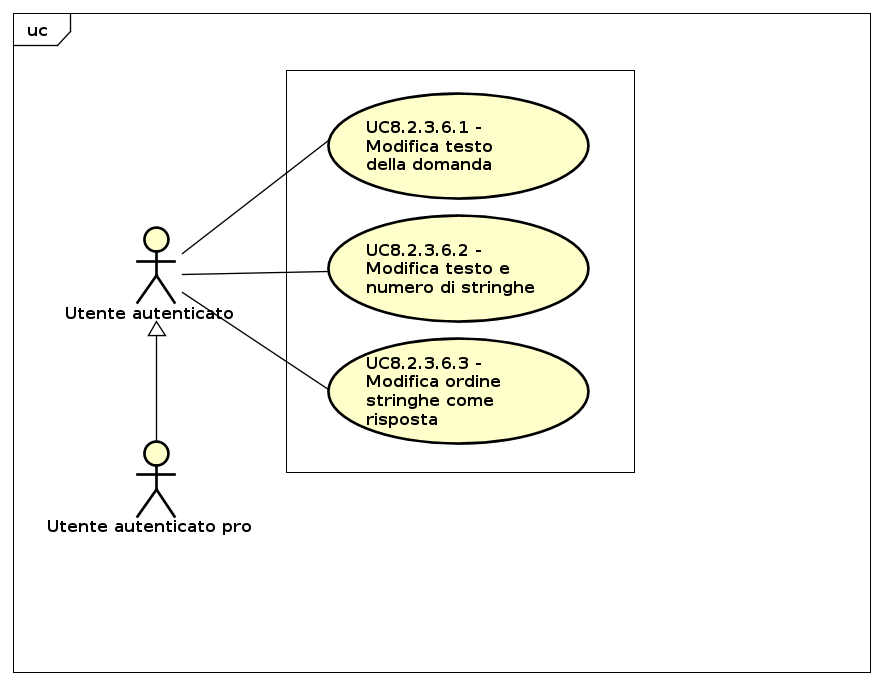
\includegraphics[scale=0.45,keepaspectratio]{UML/UC8_2_1_6.png}
		\caption{UC8.2.1.6: Modifica domanda ordinamento di stringhe}
	\end{figure}
	\FloatBarrier
\begin{itemize}
	\item\textbf{Attori}: utente autenticato, utente autenticato pro;
	\item\textbf{Descrizione}: l'attore può utilizzare la procedura guidata per la modifica di una domanda a ordinamento di stringhe;
	\item\textbf{Precondizione}: l'attore ha selezionato la funzionalità di modifica di una domanda a ordinamento di stringhe;
	\item \textbf{Postcondizione}: l'attore ha modificato una domanda a ordinamento di stringhe;
	\item\textbf{Scenario principale}:
		\begin{itemize}
			\item L'attore può modificare il testo della domanda (UC8.2.1.6.1);
			\item L'attore può modificare il testo e il numero delle stringhe che compongono la sequenza della domanda (UC8.2.1.6.2);
			\item L'attore può modificare l'ordine corretto delle stringhe che costituiscono la risposta (UC8.2.1.6.3).
		\end{itemize}
\end{itemize}

\subsubsection{Caso d'uso UC8.2.1.6.1: Modifica testo della domanda}
\begin{itemize}
	\item \textbf{Attori}: utente autenticato, utente autenticato pro;
	\item \textbf{Descrizione}: l'attore può modificare il testo della domanda;
	\item \textbf{Precondizione}: l'attore ha selezionato la funzionalità di modifica di una domanda a ordinamento di stringhe;
	\item \textbf{Postcondizione}: l'attore ha modificato il testo della domanda;
	\item \textbf{Scenario principale}: l'attore modifica il testo della domanda.
\end{itemize}

\subsubsection{Caso d'uso UC8.2.1.6.2: Modifica testo e numero di stringhe}
\begin{itemize}
	\item \textbf{Attori}: utente autenticato, utente autenticato pro;
	\item \textbf{Descrizione}: l'attore può modificare il testo e il numero di stringhe che costituiscono la risposta alla domanda;
	\item \textbf{Precondizione}: l'attore ha selezionato la funzionalità di modifica di una domanda a ordinamento di stringhe;
	\item \textbf{Postcondizione}: l'attore ha modificato il testo e il numero delle stringhe che costituiscono la risposta alla domanda;
	\item \textbf{Scenario principale}: l'attore modifica il testo e il numero delle stringhe che costituiscono la risposta alla domanda.
\end{itemize}

\subsubsection{Caso d'uso UC8.2.1.6.3: Modifica ordine stringhe come risposta}
\begin{itemize}
	\item \textbf{Attori}: utente autenticato, utente autenticato pro;
	\item \textbf{Descrizione}: l'attore può modificare l'ordine corretto delle stringhe che rappresenta la soluzione della domanda;
	\item \textbf{Precondizione}: l'attore ha selezionato la funzionalità di modifica di una domanda a ordinamento di stringhe;
	\item \textbf{Postcondizione}: l'attore ha modificato l'ordine delle stringhe che costituiscono la risposta alla domanda;
	\item \textbf{Scenario principale}: l'attore modifica l'ordine delle stringhe che costituiscono la risposta alla domanda.
\end{itemize}

\subsubsection{Caso d'uso UC8.2.1.7: Modifica domanda con area cliccabile nell'immagine}
\label{UC8.2.1.7}
\begin{figure}[h]
	\centering
	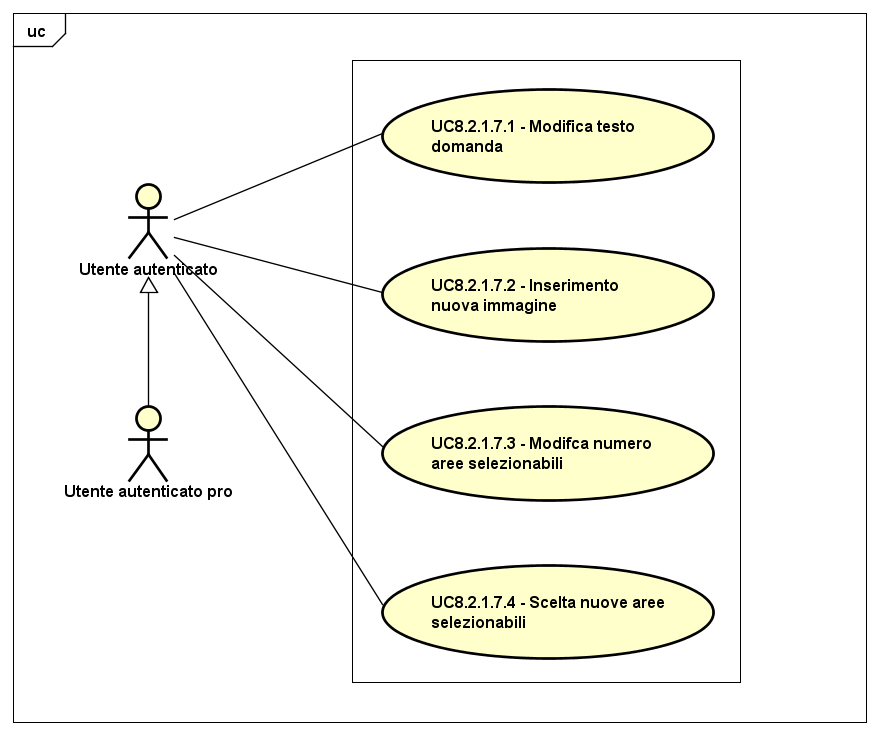
\includegraphics[scale=0.5,keepaspectratio]{UML/UC8_2_1_7.png}
	\caption{UC8.2.1.7: Modifica domanda con area cliccabile nell'immagine}
\end{figure}
\FloatBarrier
\begin{itemize}
	\item \textbf{Attori}: utente autenticato, utente autenticato pro;
	\item \textbf{Descrizione}: l'attore può utilizzare la procedura guidata per la modifica di una domanda la cui risposta è selezionabile all'interno di aree cliccabili in un'immagine;
	\item \textbf{Precondizione}: l'attore ha selezionato la modalità di modifica di una domanda con area cliccabile nell'immagine; 
	\item \textbf{Postcondizione}: l'attore ha modificato una domanda con area cliccabile nell'immagine;
	\item \textbf{Scenario principale}:
		\begin{enumerate}
	       	\item L'attore può modificare il testo della domanda (UC8.2.1.7.1);
	        \item L'attore può modificare l'immagine relativa al testo della domanda (UC8.1.1.7.2);
			\item L'attore può scegliere un nuovo numero di aree che saranno selezionabili all'interno dell'immagine (UC8.2.1.7.3);
			\item L'attore può scegliere nuove aree selezionabili all'interno dell'immagine (UC8.2.1.7.4);
	 	\end{enumerate}
\end{itemize}

\subsubsection{Caso d'uso UC8.2.1.7.1: Modifica testo della domanda}
\begin{itemize}
	\item \textbf{Attori}: utente autenticato, utente autenticato pro;
	\item \textbf{Descrizione}: l'attore può modificare il testo della domanda;
	\item \textbf{Precondizione}: l'attore ha selezionato la modalità di modifica di una domanda con area cliccabile nell'immagine; 
	\item \textbf{Postcondizione}: l'attore ha modificato il testo della domanda;
	\item \textbf{Scenario principale}: l'attore modifica il testo della domanda. 
\end{itemize}

\subsubsection{Caso d'uso UC8.2.1.7.2: Inserimento nuova immagine}
\begin{itemize}
	\item \textbf{Attori}: utente autenticato, utente autenticato pro;
	\item \textbf{Descrizione}: l'attore può inserire una nuova immagine relativa al testo della domanda che sostituisce quella già presente;
	\item \textbf{Precondizione}: l'attore ha selezionato la modalità di modifica di una domanda con area cliccabile nell'immagine;  
	\item \textbf{Postcondizione}: l'attore ha inserito una nuova immagine;
	\item \textbf{Scenario principale}: l'attore inserisce una nuova immagine al posto di quella che era presente. 	
\end{itemize}

\subsubsection{Caso d'uso UC8.2.1.7.3: Modifica numero aree selezionabili}
\begin{itemize}
	\item \textbf{Attori}: utente autenticato, utente autenticato pro;
	\item \textbf{Descrizione}: l'attore può scegliere un nuovo numero di aree selezionabili all'interno dell'immagine;
	\item \textbf{Precondizione}: l'attore ha selezionato la modalità di modifica di una domanda con area cliccabile nell'immagine; 
	\item \textbf{Postcondizione}: l'attore ha scelto il nuovo numero di aree selezionabili all'interno dell'immagine;
	\item \textbf{Scenario principale}: l'attore sceglie il nuovo numero di aree selezionabili all'interno dell'immagine. 	
\end{itemize}

\subsubsection{Caso d'uso UC8.2.1.7.4: Modifica aree selezionabili}
\begin{itemize}
	\item \textbf{Attori}: utente autenticato, utente autenticato pro;
	\item \textbf{Descrizione}: l'attore può scegliere dove inserire le nuove aree selezionabili o riposizionare quelle già presenti all'interno dell'immagine;
	\item \textbf{Precondizione}: l'attore ha selezionato la modalità di modifica di una domanda con area cliccabile nell'immagine; 
	\item \textbf{Postcondizione}: l'attore ha scelto dove inserire le nuove aree selezionabili o dove riposizionare quelle già presenti all'interno dell'immagine;
	\item \textbf{Scenario principale}: l'attore sceglie dove inserire le nuove aree selezionabili o riposiziona quelle già presenti all'interno dell'immagine. 	
\end{itemize}



	\subsubsection{Caso d'uso UC8.2.2: Conferma modifica}
	\begin{itemize}
		\item
			\textbf{Attori}: utente autenticato, utente autenticato pro;
		\item
			\textbf{Descrizione}: l'attore può confermare la modifica della domanda;
		\item		
			\textbf{Precondizione}: l'attore ha finito di modificare una domanda tramite un wizard;
		\item
			\textbf{Postcondizione}: l'attore ha modificato una domanda;
		\item
			\textbf{Scenario principale}: l'attore conferma la modifica della domanda;		
		\item
	 		\textbf{Scenari alternativi}: l'attore annulla la modifica della domanda.
	\end{itemize}		
	\subsubsection{Caso d'uso UC8.2.3: Visualizzazione errore modifica}
	\begin{itemize}
		\item
			\textbf{Attori}: utente autenticato, utente autenticato pro;
		\item
			\textbf{Descrizione}: l'attore può visualizzare un messaggio d'errore nel caso si fossero verificati uno o più scenari alternativi durante la modifica della domanda;
		\item		
			\textbf{Precondizione}: il sistema ha ricevuto dei dati errati per la modifica della domanda;
		\item
			\textbf{Postcondizione}: il sistema avvisa l'attore dell'errore verificatosi tramite un opportuno messaggio;
		\item
			\textbf{Scenario principale}: l'attore visualizza un messaggio d'errore.	
	\end{itemize}	